\documentclass[10pt,a4paper]{report}
\usepackage[utf8]{inputenc}
\usepackage{amsmath}
\usepackage{amsfonts}
\usepackage{amssymb}
\usepackage{graphicx}
\usepackage{pgfplots}
\usepackage{pgfplotstable}

\usepackage{fancyhdr}
\usepackage{graphicx}
\usepackage{epstopdf}

\usepackage{placeins}

\usepackage{hyperref}

\usetikzlibrary{pgfplots.groupplots}

%\usepackage{struktex}
\usepackage{hyperref}
\hypersetup{
    colorlinks=true,
    linkcolor=blue,
    urlcolor=red,
    linktoc=all
}

\graphicspath{{./}}

\usepackage[left=1.5cm,right=1.5cm,top=2cm,bottom=2cm]{geometry}



\definecolor{s1_1}{RGB}{38,70,83}
\definecolor{s1_2}{RGB}{42,157,143}
\definecolor{s1_3}{RGB}{233,196,106}
\definecolor{s1_4}{RGB}{244,162,97}
\definecolor{s1_5}{RGB}{231,111,81}

\definecolor{s2_1}{RGB}{246,81,29}
\definecolor{s2_2}{RGB}{255,180,0}
\definecolor{s2_3}{RGB}{0,166,237}
\definecolor{s2_4}{RGB}{127,184,0}
\definecolor{s2_5}{RGB}{13,44,84}



\pgfplotscreateplotcyclelist{convergelist}{
s2_1, thick, solid, mark=*\\%
s2_2, thick, solid, mark=square\\%
s2_3, thick, solid, mark=diamond*\\%
s2_4, thick, solid, mark=triangle\\%
s2_5, thick, solid, mark=asterisk\\%
}

\pgfplotscreateplotcyclelist{elelist}{
s2_1, solid\\%
s2_2, solid\\%
s2_3, solid\\%
s2_4, solid\\%
s2_5, solid\\%
}




\def \resultspath {../results}
\def \pathpartone {../../1_three-dimensional_atomic_system}
\def \pathparttwo {../../2_Two-dimensional_atomic_tensile_test}
\def \fullpathpartone {/home/lukas/Desktop/project/independence/atomistic_modeling/exam/1_three-dimensional_atomic_system}
\def \fullpathparttwo {/home/lukas/Desktop/project/independence/atomistic_modeling/exam/2_Two-dimensional_atomic_tensile_test}


\newcommand{\dvec}[1]{\boldsymbol{ \mathsf{#1} } }         % for vectors
\newcommand{\dmat}[1]{\boldsymbol{\mathsf{#1}}}           % for matrices
\newcommand{\Bd}[2]{ (#1,#2)_{D^k} }           % bilienarfor over domian
\newcommand{\Bb}[2]{ (#1,#2)_{\partial D^k} }           % bilienarfor over boundary

\newcommand{\pd}{\partial}
\newcommand{\pdfrac}[2]{\frac{\pd #1}{\pd #2}}  



\title{Report Project 2}
\author{Lukas Scheucher}



\pgfplotstableset{
  col sep=comma,
    create on use/X/.style={create col/copy column from table={/home/lukas/LRZ Sync+Share/Studium/Fach/DG/DG_project/lukas/results/config_task3_K5_N1_LF_x.dat}{0}}
}



\begin{document}


\chapter{Three-dimensional atomistic system}
For the determination of the lattice constant and lattice type, 3 different configurations are considered:
\begin{enumerate}
\item Face-centered cubic (FCC)
\item Body-centered cubic (BCC)
\item Primitive cubic     (PC)
\end{enumerate}
The system will take those configuration, which shows the least total energy per atom. Since interactions happen not only with the closes neighbors, but also with other atoms, an simulation has to be performed to get the exact energies.\\
However, a good first approximation can be made analytically by considering the following observations: All atoms within a lattice type are equal, meaning that an atom that appears as a center atom in BCC can also be viewed as a corner atom just by shifting the connections. Secondly, if one denoted the length of the cube as lattice constant $a$, one can easily determine the distances between all atom by simple geometric means.\\
By looking only at the closest neighbors, one can derive the following expression for the energy per atom in all 3 grids:
\begin{align}
E_{FCC}&=6 U(a_{FCC})+12 U(a_{FCC}/\sqrt{2}) \\
E_{BCC}&=6 U(a_{BCC})+8 U(a_{BCC} \sqrt{3}/2) \\
E_{PC} &=6 U(a_{PC})
\end{align}

By solving for local minima, the following lattice constants are obtained
\begin{align}
a_{FCC,min}&= 5.7432\AA\\
a_{BCC,min}&= 4.6143\AA\\
a_{PC,min} &= 4.097\AA\\
\end{align}

Substituting this back in to the equation for the energies per atom, one can see, that the FCC configuration with an approximate lattice constant of $5.7432\AA$ gives the smallest total energy and is therefore the configuration obtained.\\

Scripts used for this question:
\href{../../lattice_constant_approximation.m}{lattice\_constant\_approximation.m}


Of course, the lattice constant can also be obtained by simulations. This has been done with the input script \href{../../DIR1/in.latticeconstant}{in.latticeconstant}. To run the simulations just call \href{../../DIR1/run_latticeconstant.sh}{run\_latticeconstant.sh}.\\
The lattice-constant obtained after minimization is $5.64 \AA$. The minimization process is visualized in Figure~\ref{fig:p1_latticeconst}.

\begin{center}
\begin{figure}[h]
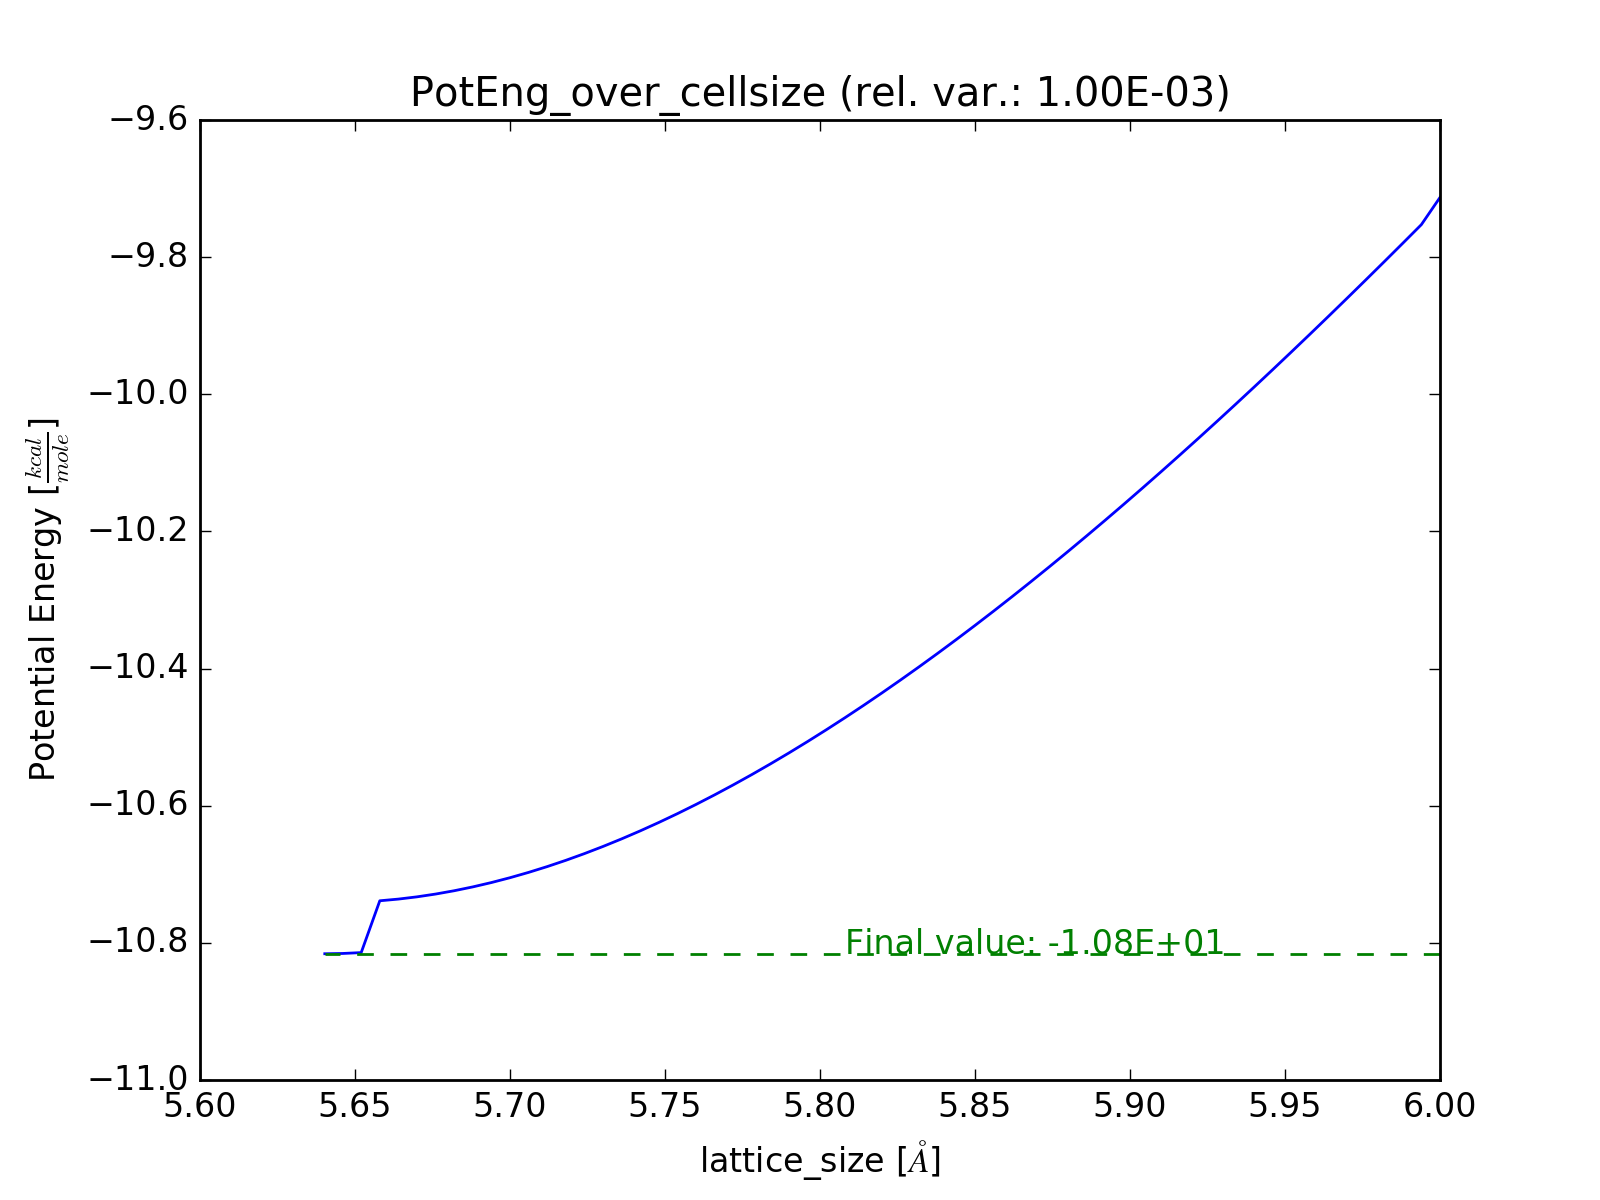
\includegraphics[width=0.5\textwidth]{\fullpathpartone/plots/latticeconst/PotEng_over_Lx.png}~
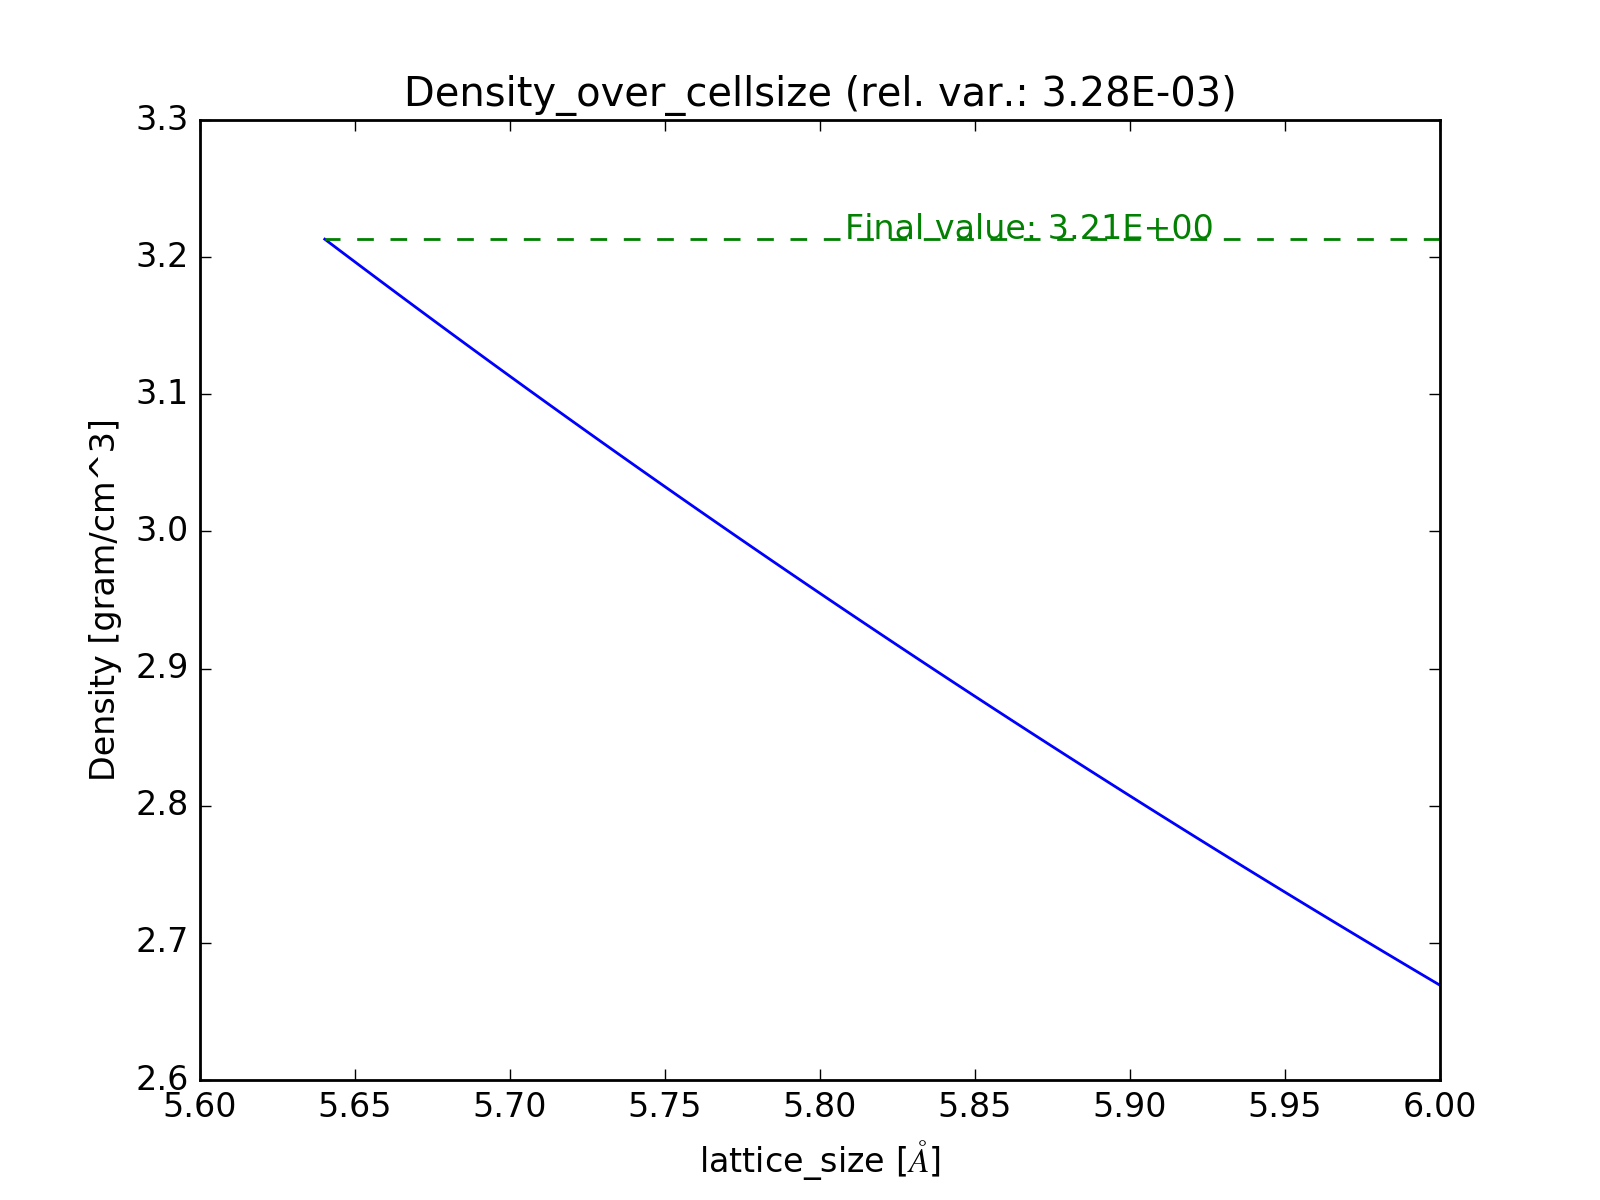
\includegraphics[width=0.5\textwidth]{\fullpathpartone/plots/latticeconst/Density_over_Lx.png}~
\caption[aa]{Convergence of Potential energy on the left, Final density value on the right. The final lattice-constant determined by the simulation is \textbf{5.640 $\AA$}. }
\label{fig:p1_latticeconst}
\end{figure}
\end{center}


\section{Constant temperature and molecular dynamics}
Through several simulations, a timestep of $10 fs$ has been determined as stable. The input-files for all simulations are \href{\pathpartone/in.NVT_template}{in.NVT\_template} for the Noose-Hover thermostat and \href{\pathpartone/in.NVEBer_template}{in.NVEBer\_template} for the "weak-coupling" Berendsen thermostat.

\subsection{Equilibriation}
For the equilibriation phase, the lattice constant of $5.90 \AA$, as states on the instruction, has been used. The results are plotted in Figure~\ref{fig:p1_equilibriation}. All relative variances have been calculated after the system has reached equilibrium. The plots show, that the weakly coupled Berendsen thermostat capable of delivering the exact temperature value. However, while damping helps to reduce the fluctuation in Potential energy, it increases the variance of the temperature values. For the NVT thermostat on the other hand, damping can help to reduce fluctuations in all quantities of interest.\\
Overall, the weakly-coupled Berendsen thermostat clearly performs superior compared to Nose-Hoover.

\begin{center}
\begin{figure}[h]
g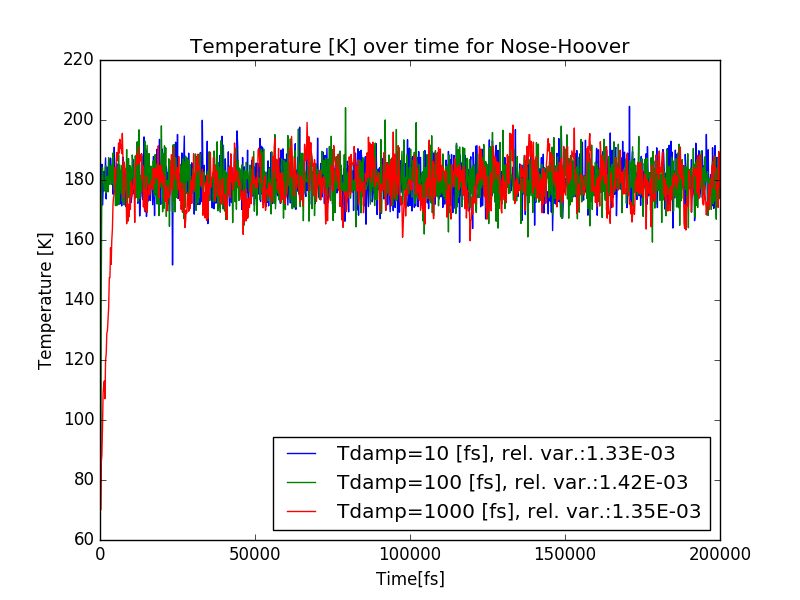
\includegraphics[width=0.5\textwidth]{\fullpathpartone/plots/dampstudy/NVT_Temp_atomnum500.png}~
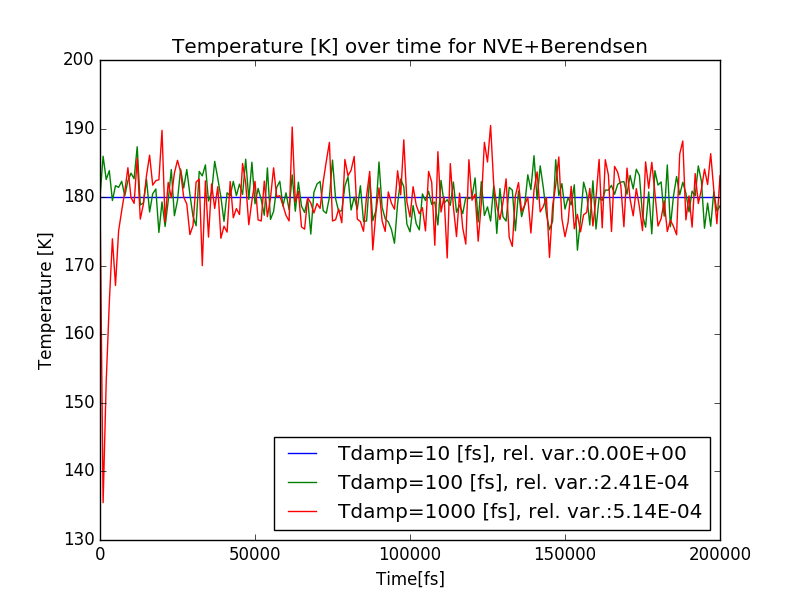
\includegraphics[width=0.5\textwidth]{\fullpathpartone/plots/dampstudy/NVEBer_Temp_atomnum500.png}
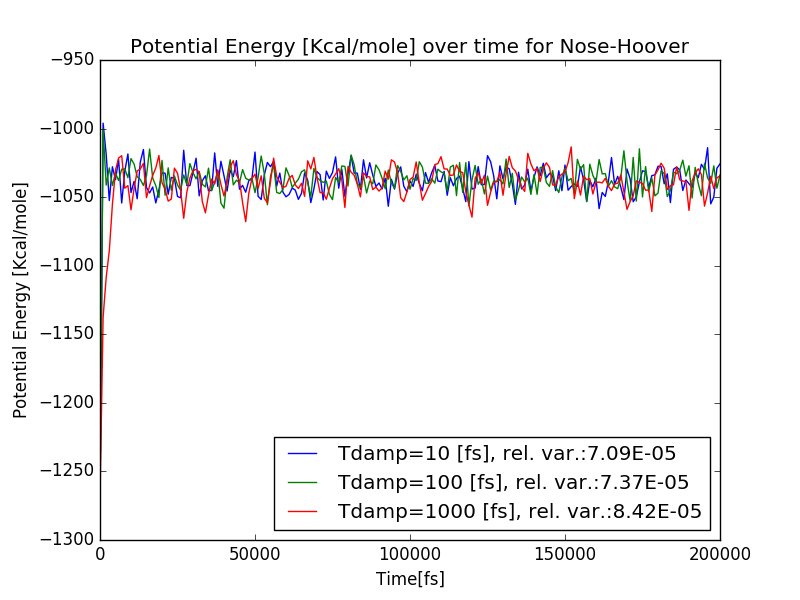
\includegraphics[width=0.5\textwidth]{\fullpathpartone/plots/dampstudy/NVT_PotEng_atomnum500.png}~
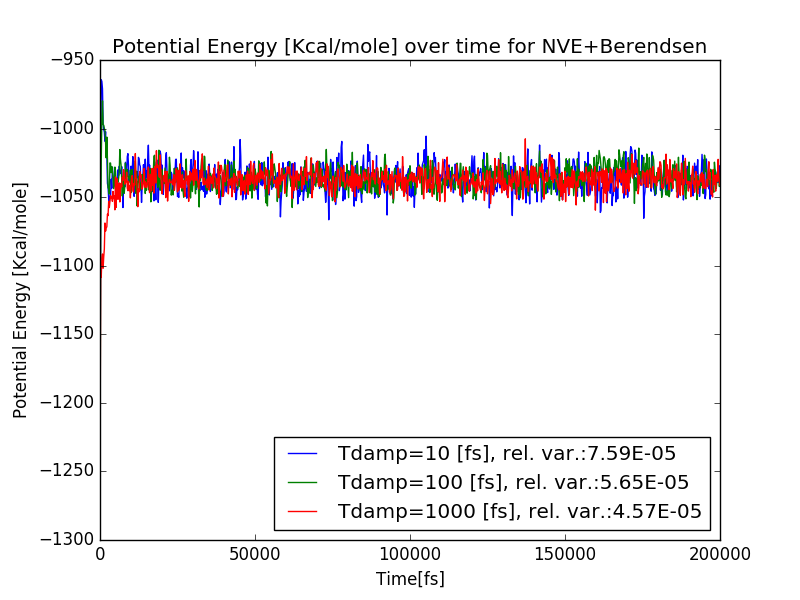
\includegraphics[width=0.5\textwidth]{\fullpathpartone/plots/dampstudy/NVEBer_PotEng_atomnum500.png}
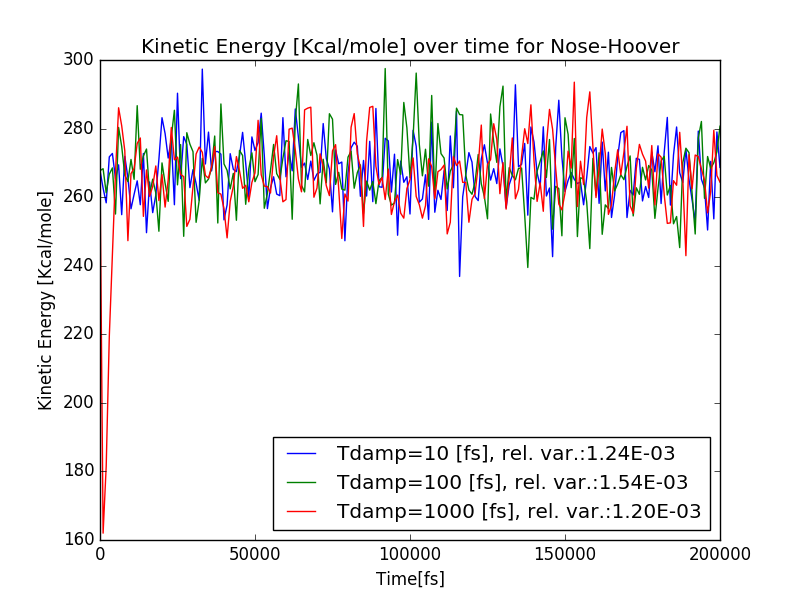
\includegraphics[width=0.5\textwidth]{\fullpathpartone/plots/dampstudy/NVT_KinEng_atomnum500.png}~
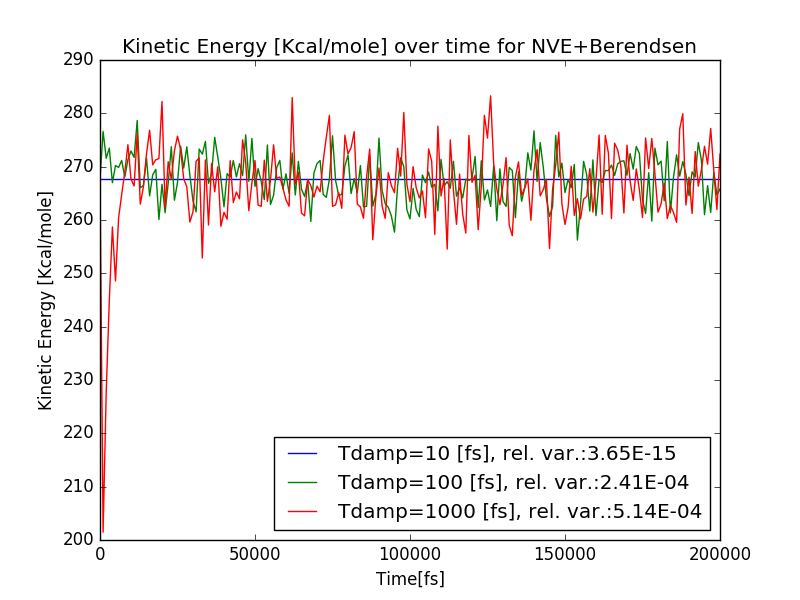
\includegraphics[width=0.5\textwidth]{\fullpathpartone/plots/dampstudy/NVEBer_KinEng_atomnum500.png}
\caption[aaa]{Equilibration of Temperature(top), Potential Energy(middle) and Kinetic Energy(bottom) for the Nose-Hoover thermostat(left) and the "weak-coupling" thermostat(right). The equilibriation is plotted for different damping parameters and the relative variance of the equilibrated part is provided.}
\label{fig:p1_equilibriation}
\end{figure}
\end{center}


\subsection{Stability comparison between Noose-Hoover and Berendsen}
A comparison between the Nose-Hoover thermostat and the weakly-coupled Berendsen thermostat is provided in Figure~\ref{fig:p1_NVT_vs_NVEBer}.
Overall, one can say that the weakly-coupled Berendsen delivers more accurate and stable results. Also, it does not benefit from damping, on the contrary, the relative variance increases with an increasing damping parameter.

\begin{center}
\begin{figure}[h]
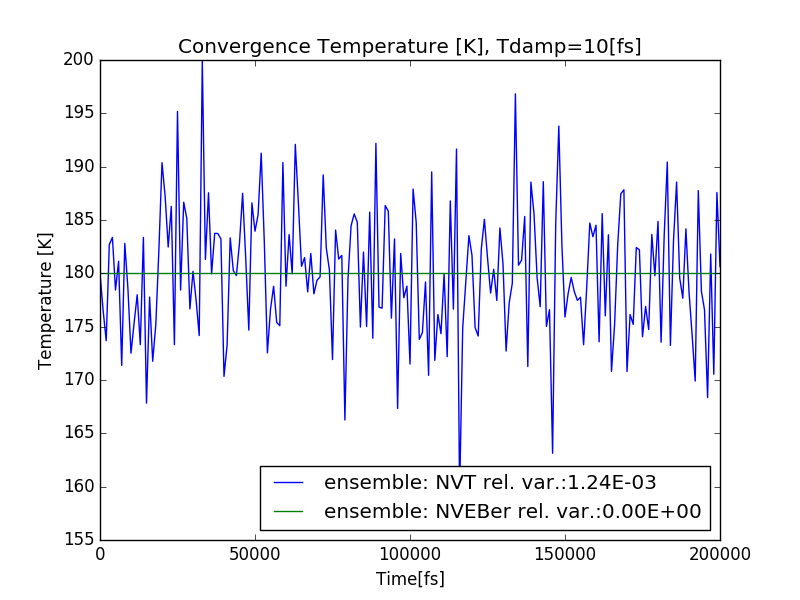
\includegraphics[width=0.5\textwidth]{\fullpathpartone/plots/NVT_vs_NVEBer/Temp_damp10_atomnum500.png}~
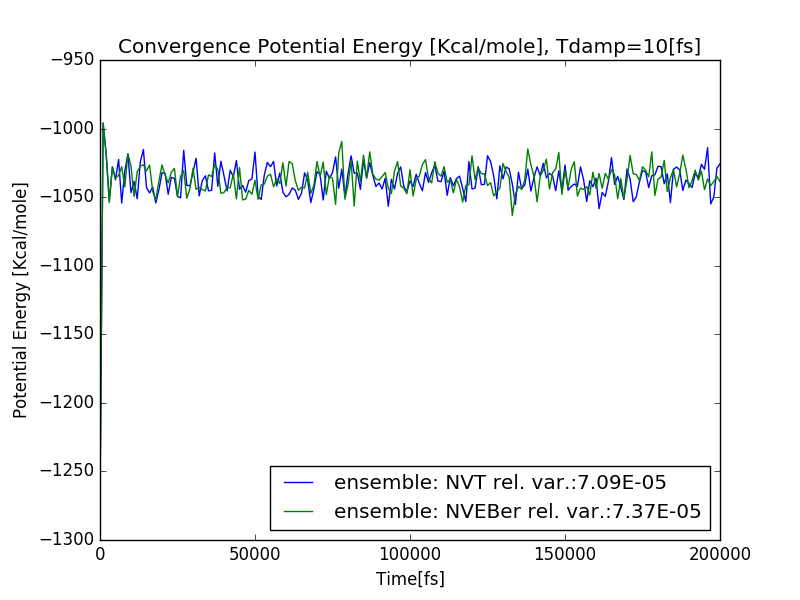
\includegraphics[width=0.5\textwidth]{\fullpathpartone/plots/NVT_vs_NVEBer/PotEng_damp10_atomnum500.png}
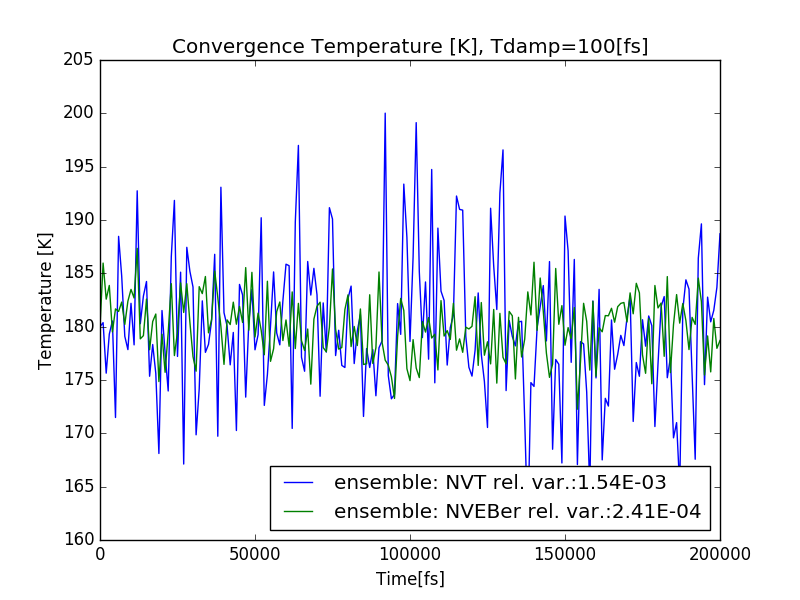
\includegraphics[width=0.5\textwidth]{\fullpathpartone/plots/NVT_vs_NVEBer/Temp_damp100_atomnum500.png}~
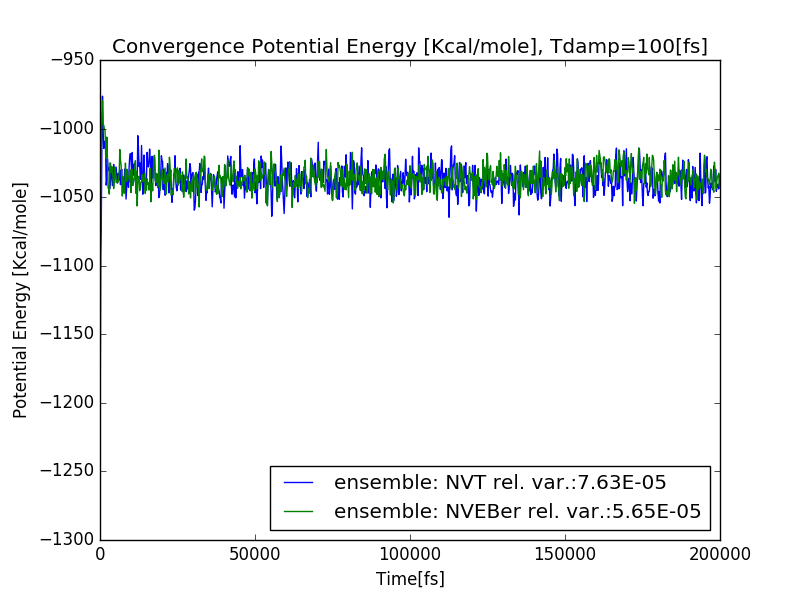
\includegraphics[width=0.5\textwidth]{\fullpathpartone/plots/NVT_vs_NVEBer/PotEng_damp100_atomnum500.png}
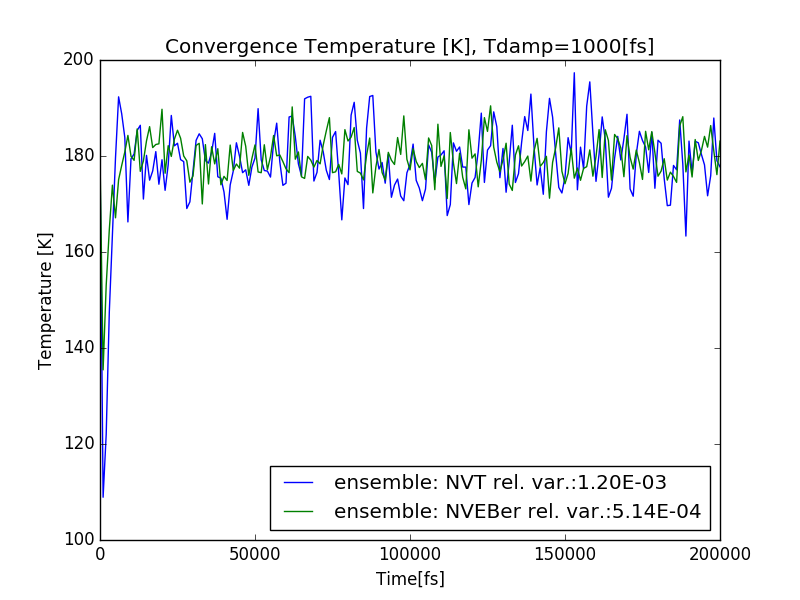
\includegraphics[width=0.5\textwidth]{\fullpathpartone/plots/NVT_vs_NVEBer/Temp_damp1000_atomnum500.png}~
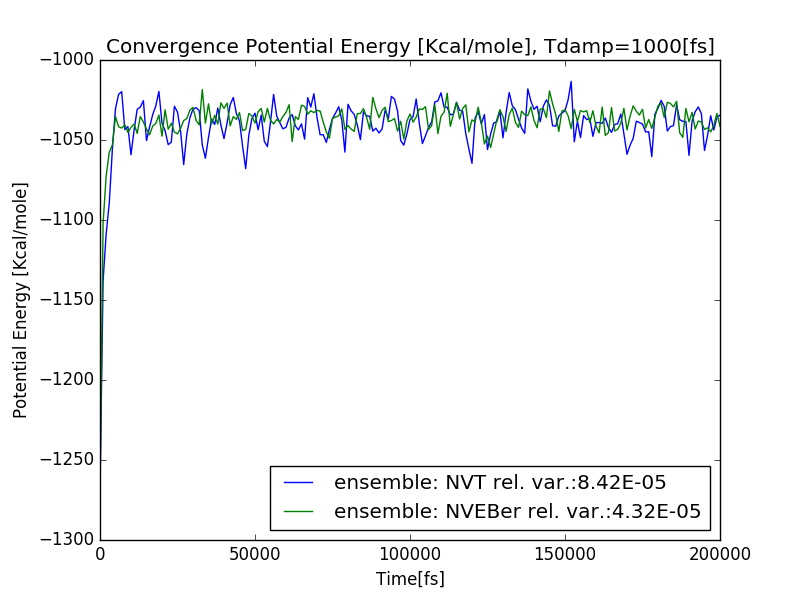
\includegraphics[width=0.5\textwidth]{\fullpathpartone/plots/NVT_vs_NVEBer/PotEng_damp1000_atomnum500.png}
\caption[aaa]{Comparisons between Nose-Hoover thermostat(blue) and weakly-coupled Berendsen(green) for temperature (left) and Potential Energy(right). The 3 rows show the convergence for 3 different damping parameters.}
\label{fig:p1_NVT_vs_NVEBer}
\end{figure}
\end{center}


\subsection{Dependence on the system-size}
To determine the dependence of the Nose-Hoover thermostat's convergence on the system size, simulations with a box-size of 5, 6, 7, 8, 9, 10, 11 and 12 have been carried out, which correlates to a total number of atoms of 500, 864, 1372, 2048, 2916, 4000, 5324 and 6912. The results are visualized in Figure~\ref{fig:p1_cellnum_study}. It can be observed, that the relative variance decays with the system size as $\frac{<T^2>-<T>^2}{<T>^2}\sim\frac{1}{N}$.

\begin{center}
\begin{figure}[h]
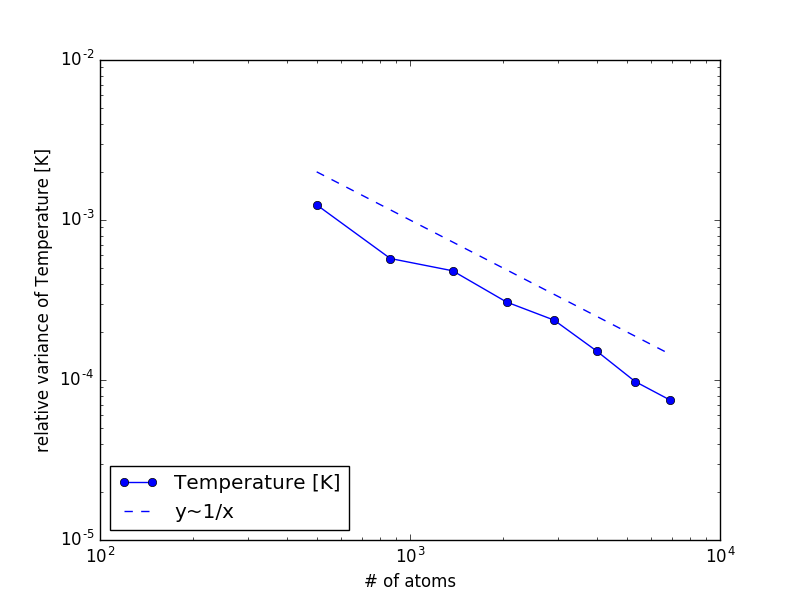
\includegraphics[width=0.5\textwidth]{\fullpathpartone/plots/cellnum_study/NVT_Temp_damp10.png}
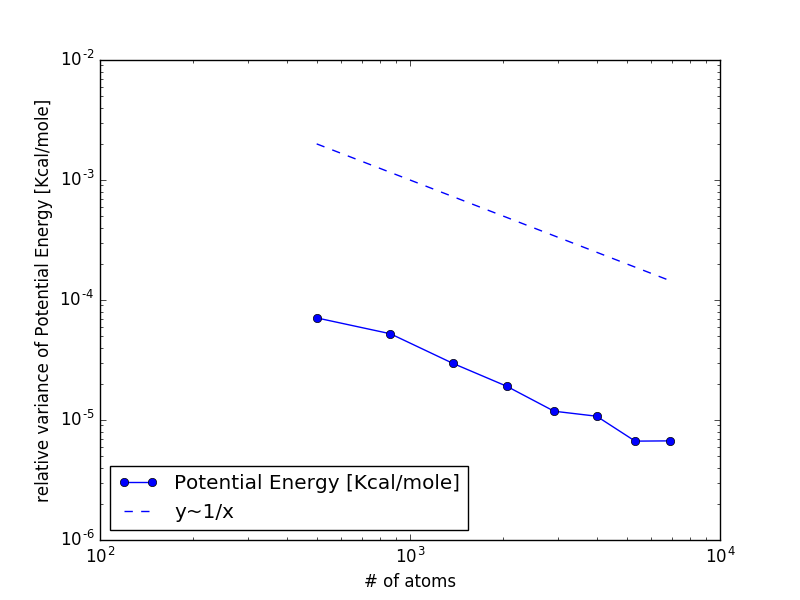
\includegraphics[width=0.5\textwidth]{\fullpathpartone/plots/cellnum_study/NVT_PotEng_damp10.png}
\caption[aaa]{Relative variance of Temperature(left) and Potential Energy(right) with respect to the number of atoms in the simulation. As the dashed line shows, the relative variance decays with the system size as $\frac{<T^2>-<T>^2}{<T>^2}\sim\frac{1}{N}$.}
\label{fig:p1_cellnum_study}
\end{figure}
\end{center}


\subsection{MCMC}
The inputfile for the MCMC simulations was \href{\pathpartone/in.NVT_MCMC}{in.NVT\_MCMC}, the simulations were run by \href{\pathpartone/run_NVT_MCMC.sh}{run\_NVT\_MCMC.sh}, results were posprocessed with \href{\pathpartone/postprocess_MCMC.sh}{postprocess\_MCMC.sh} and plotted via \href{\pathpartone/plot_MCMC_vs_NVT.py}{plot\_MCMC\_vs\_NVT.py}.
The results are stored in \href{\pathpartone/plots/MCMC_vs_NVT/}{plots/MCMC\_vs\_NVT/}.\\
A visualization of the Density and Potential Energy results in provided in Figure\ref{fig:p1_MCMC_vs_NVT}.\\
MCMC converges a little bit faster, but other than that neither the relative variance, nor the final distribution obtained are diffferent. For this reason, I conclude that in this setup, the performance of MCMC does not justify the significantly increased cost.

\subsubsection{Difference between MCMC and MD}
Molecular dynamics is based on the solution of simple ODEs of motion for every particle. A time integrator is applied to move the system from time $t^n$ to $t^n$ plus one. The most csotly part of MCMC is the evaluation of the force on a particle, since all neighbour interactions must be taken into account(up to a defined cutoff radius). Also, parallelization is limited, since neighbouring regions have to continously exchange information about the particles on the border.\\
For MCMC, no neighbour evaluations are required. Instead, every particles position(momenta) is subsequantly updated by computing the Markov chain. MCMC can be advantagous for very large systems and high dimensions, in the examle here, it could not utilize its advantages.


\begin{center}
\begin{figure}[h]
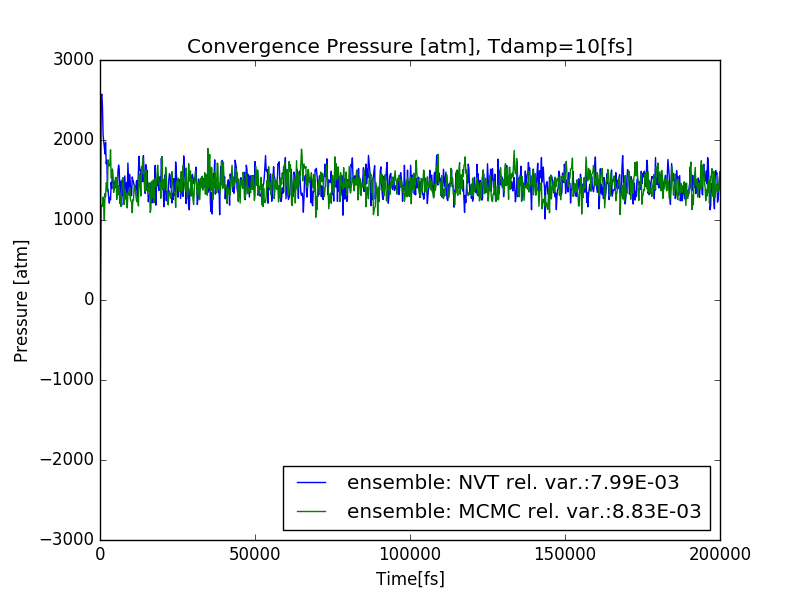
\includegraphics[width=0.5\textwidth]{\fullpathpartone/plots/MCMC_vs_NVT/Press_damp10.png}~
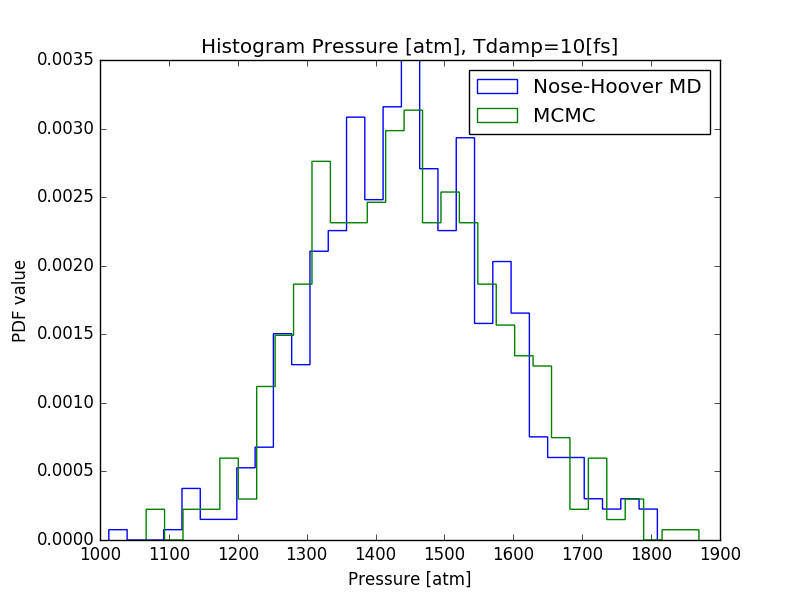
\includegraphics[width=0.5\textwidth]{\fullpathpartone/plots/MCMC_vs_NVT/hist_Press_damp10.png}
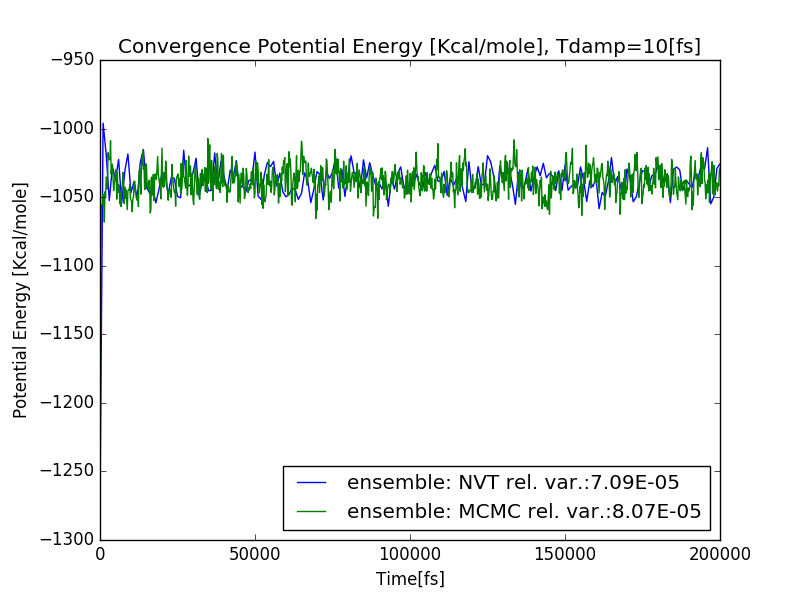
\includegraphics[width=0.5\textwidth]{\fullpathpartone/plots/MCMC_vs_NVT/PotEng_damp10.png}~
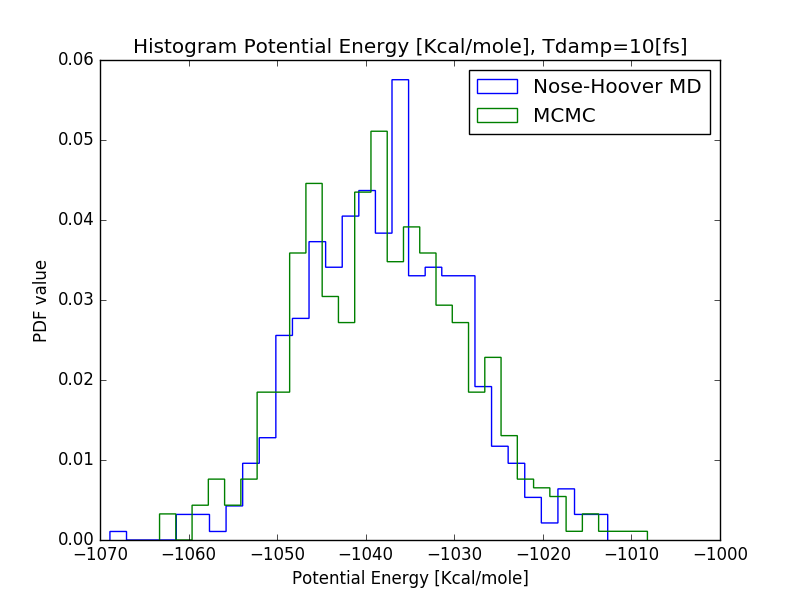
\includegraphics[width=0.5\textwidth]{\fullpathpartone/plots/MCMC_vs_NVT/hist_PotEng_damp10.png}
\caption[aaa]{Comparison between MCMC and NVT-MD. Boit algorithms deliver very similar results. MCMC converges a little bit faster, but other than that neither the relative variance, nor the final distribution obtained are diffferent.}
\label{fig:p1_MCMC_vs_NVT}
\end{figure}
\end{center}








\section{Constant pressure/temperature molecular dynamics}
\subsection{Finding the equilibrium box sizes}
To determine the equilibrium box sizes, a regular simulation has been conducted and the final, equilibrium average has been used as a mean value. This is visualized in Figure~\ref{fig:p1_boxsize}. By dividing the final box-length by the original, one can obtain a scaling factor that is applied to the following simulations via the "change\_box" command(\href{\pathpartone/in.NPT_boxmod_template}{in.NPT\_boxmod\_template}).
As a verification, the box-size is again plotted over time in the right hand side of Figure~\ref{fig:p1_boxsize}.\\

In Figure~\ref{fig:pressure_over_boxsize}, the pressure distribution of the scaled simulation is plotted for different box sizes. We can clearly see a normal-like distribution centered around the target value of 1.0 atm and a shrinking variance with increasing system size.\\
The dependency of the relative variance on the number of atoms is also plotted in the bottom two figures. Clearly, the relative variance decays inverse proportional with the system size.\\
 \\
From the LAMMPS manual, we can see that the pressure is computes via the formula
\begin{align}
P=\frac{N k_B T}{N}+\frac{\sum_i^{N'}r_i\cdot f_i}{dV}
\end{align}
where $N$ is the number of atoms $k_B$ is the Boltzmann constant, $T$ is the Temperature and $V$ is the control volume. The second term contains all interactions where $r_i$ and $f_i$ are the position vector if atom $i$ and dV is the change rate of the control volume. Since we are in equilibrium, the control volume remains constant, the second term can thus be neglected. Also, in the first term, $\frac{N}{V}$ is related to the density and also constant. We can therefore expect the convergence to be of the same rate as the convergence of $T$ which has already been shown in the first part to be of first order.


\begin{center}
\begin{figure}[h]
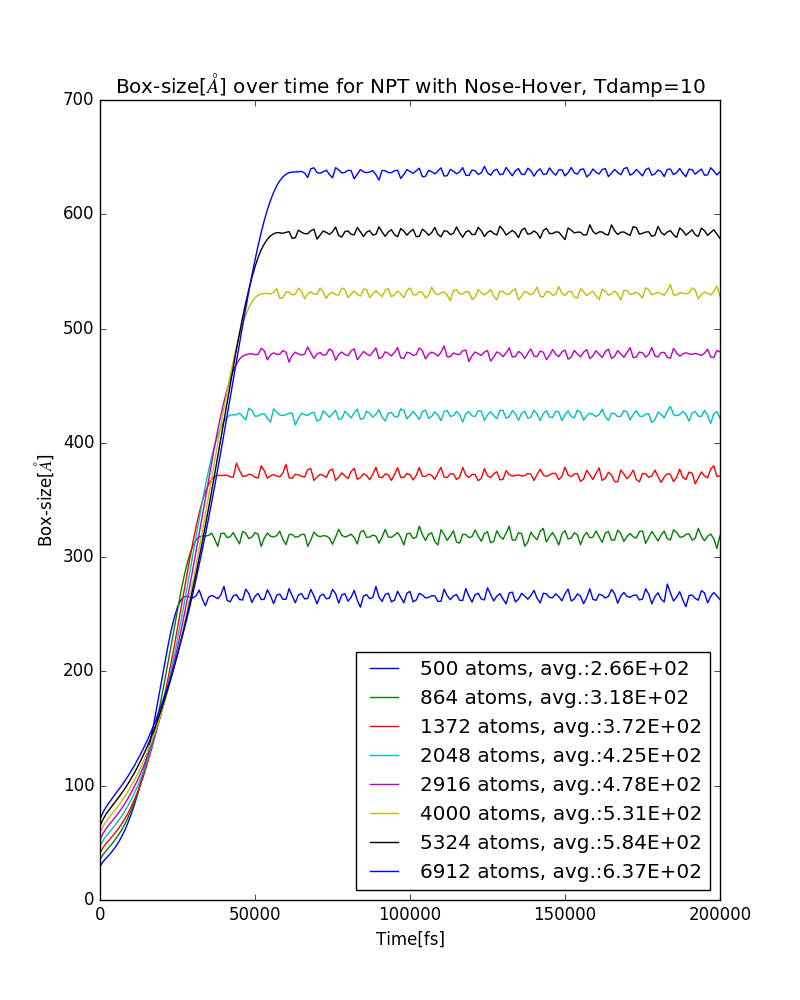
\includegraphics[width=0.5\textwidth]{\fullpathpartone/plots/boxsizesim/NPT_Lx_damp10.png}~
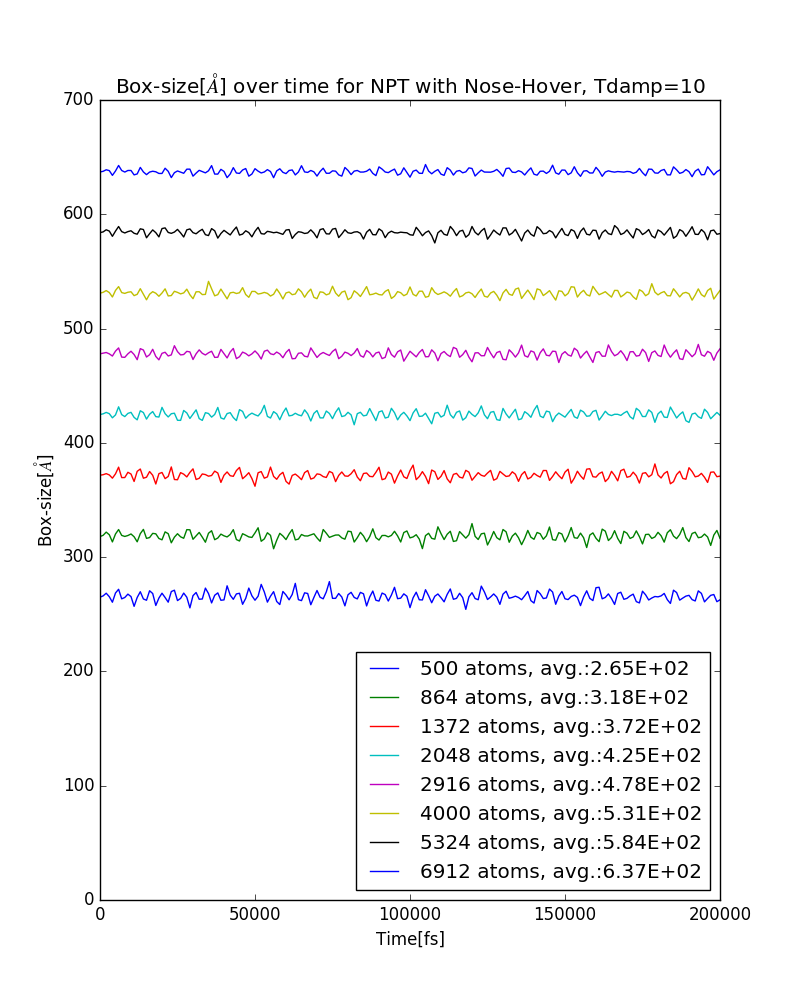
\includegraphics[width=0.5\textwidth]{\fullpathpartone/plots/boxsizesim/boxmod_NPT_Lx_damp10.png}
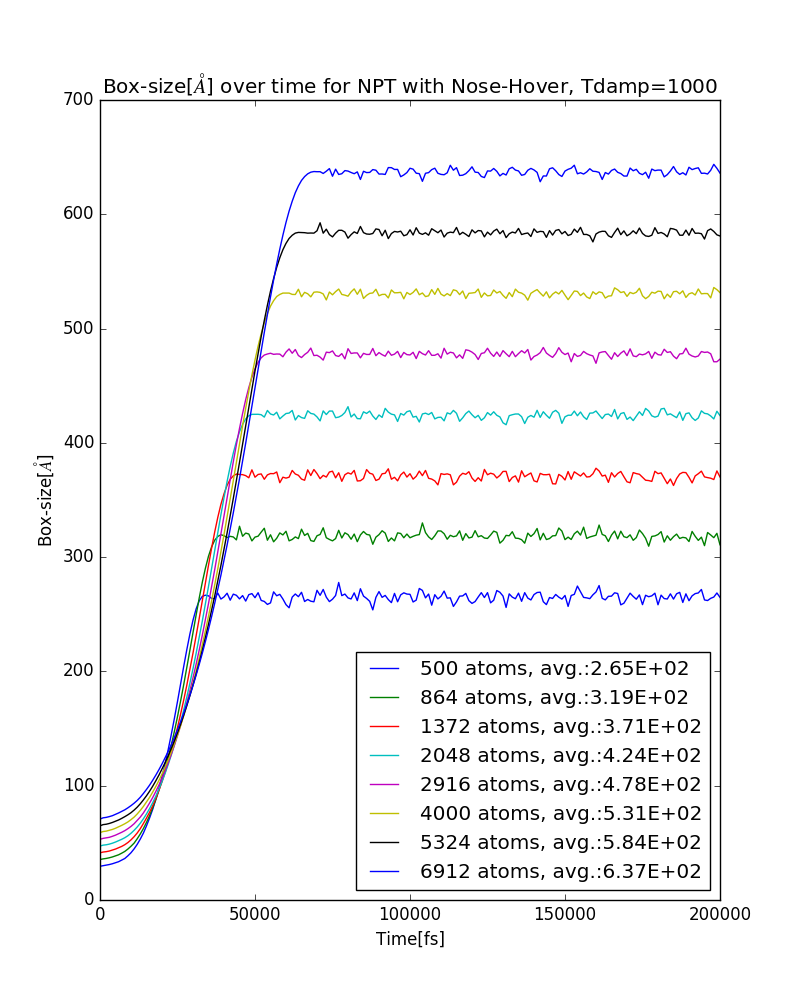
\includegraphics[width=0.5\textwidth]{\fullpathpartone/plots/boxsizesim/NPT_Lx_damp1000.png}~
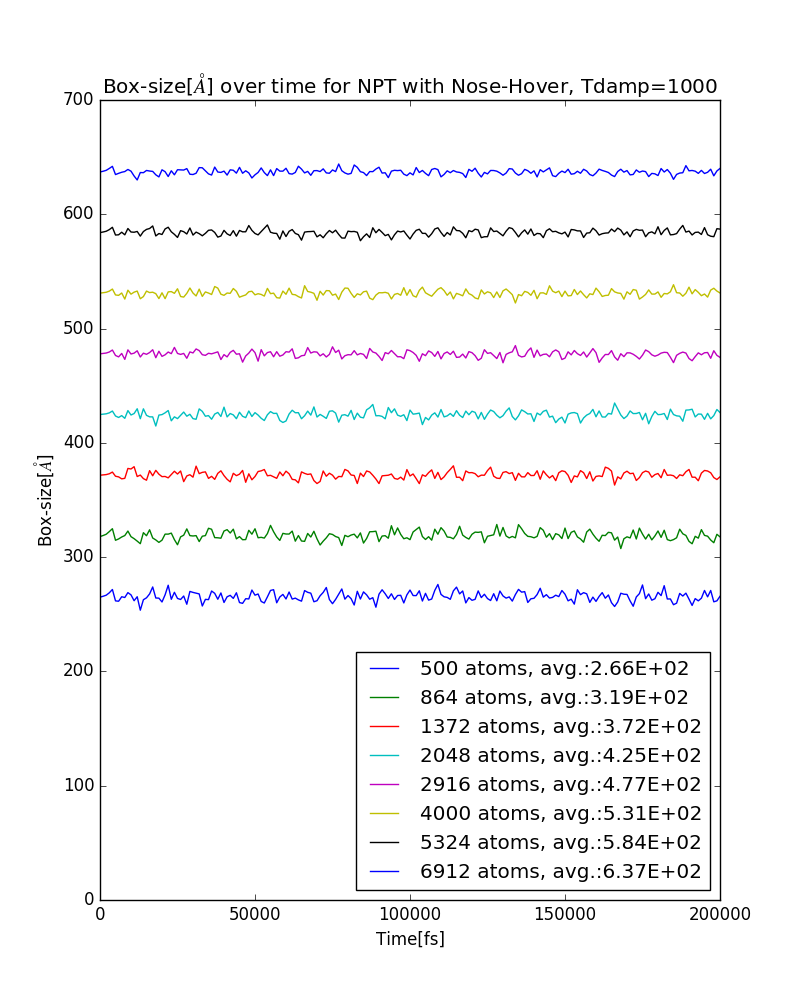
\includegraphics[width=0.5\textwidth]{\fullpathpartone/plots/boxsizesim/boxmod_NPT_Lx_damp1000.png}
\caption[aaa]{Determination of the box-size by equilibriation(left) and Time convergence after box-size modification (right). }
\label{fig:p1_boxsize}
\end{figure}
\end{center}


\begin{center}
\begin{figure}[h]
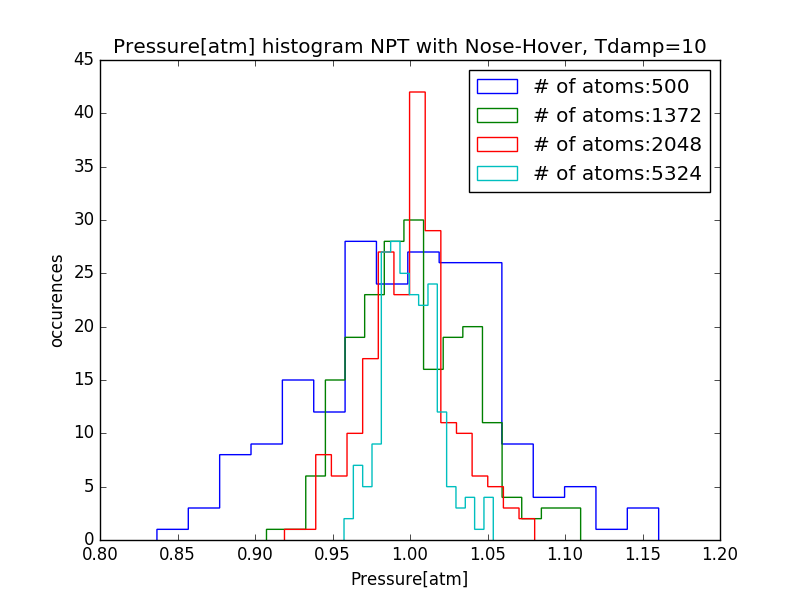
\includegraphics[width=0.5\textwidth]{\fullpathpartone/plots/boxsizesim/boxmod_NPT_Press_damp10.png}~
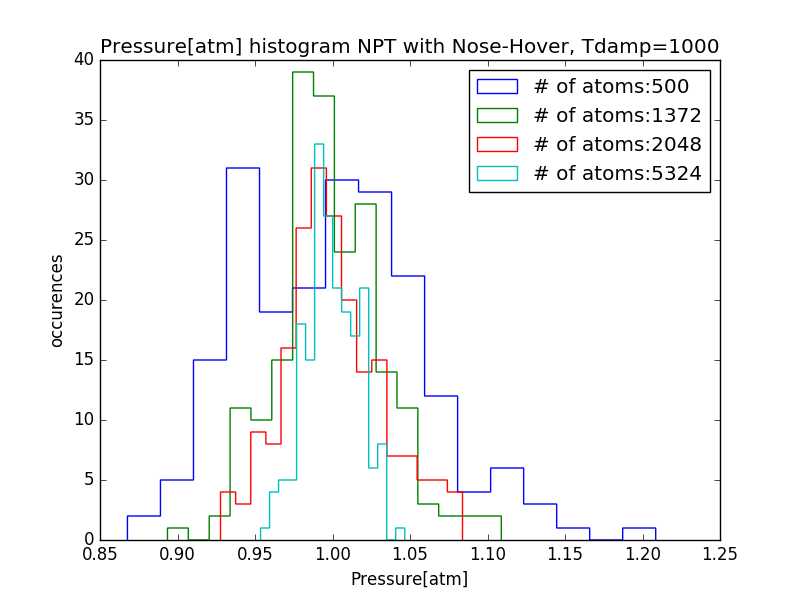
\includegraphics[width=0.5\textwidth]{\fullpathpartone/plots/boxsizesim/boxmod_NPT_Press_damp1000.png}
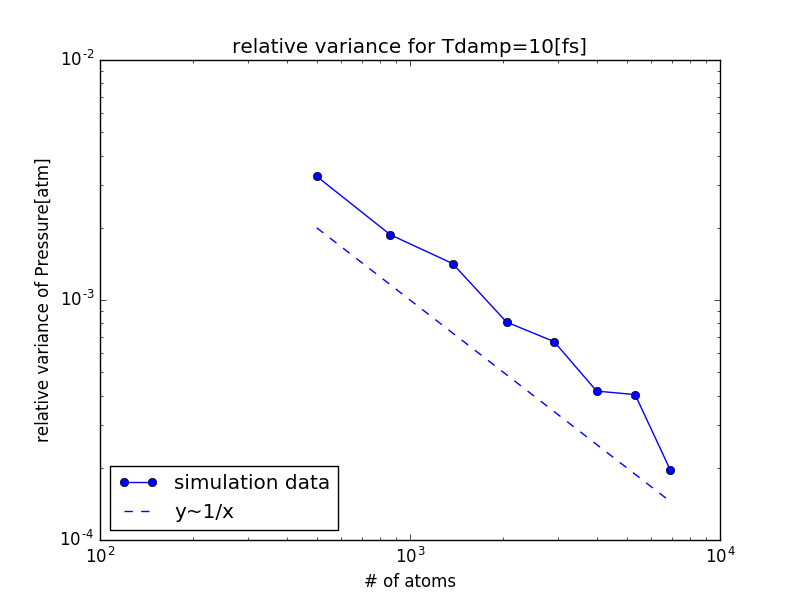
\includegraphics[width=0.5\textwidth]{\fullpathpartone/plots/boxsizesim/relvar_Press_damp10.png}~
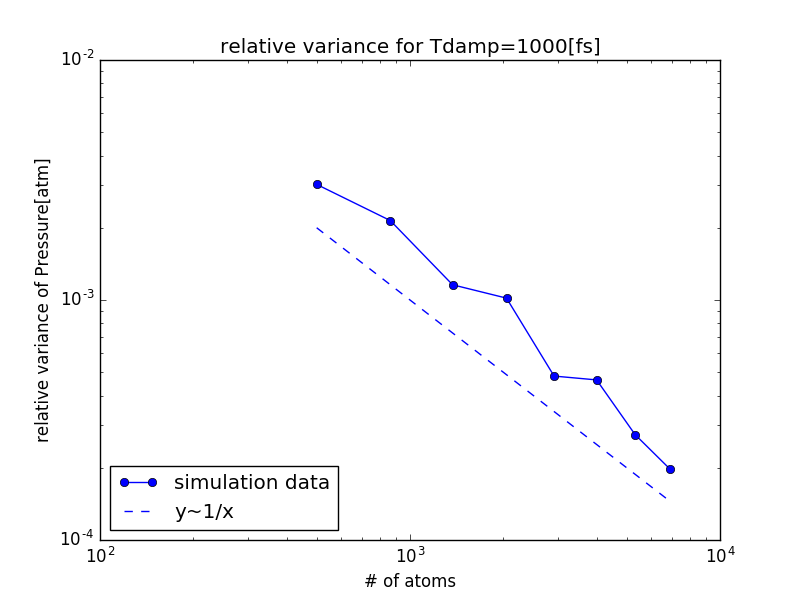
\includegraphics[width=0.5\textwidth]{\fullpathpartone/plots/boxsizesim/relvar_Press_damp1000.png}
\caption[aaa]{Influence of the system size on the simulation. The top two figures show histograms of the obtained pressure values, the bottom two figures show the dependency of the relative variance on the system size. The left two figures have been calculated with a damping value of $10 fs$ the right two with $1000 fs$.}
\label{fig:pressure_over_boxsize}
\end{figure}
\end{center}


\begin{center}
\begin{figure}[h]
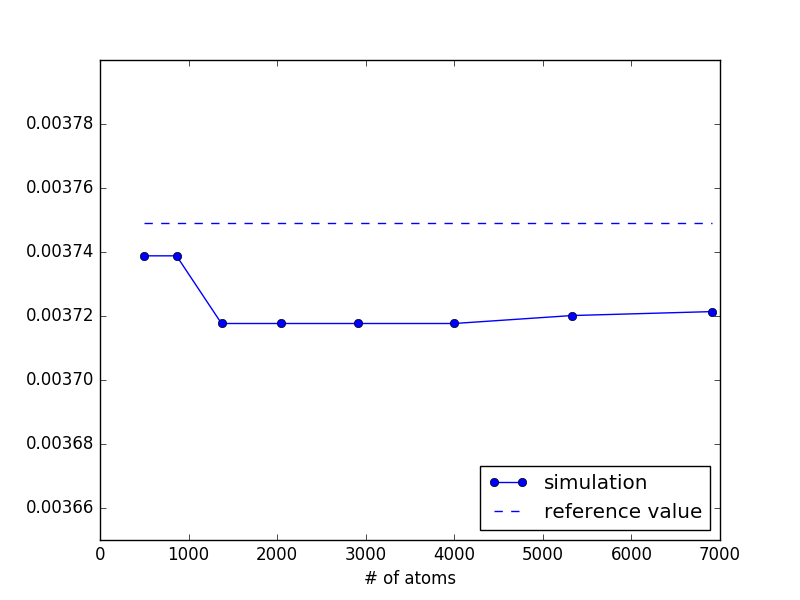
\includegraphics[width=0.5\textwidth]{\fullpathpartone/plots/boxsizesim/boxmod_NPT_Density_damp10.png}~
\caption[aaa]{Density results as a function of the simulation box size. Clearly, the reference density is very well approximated. On should also take into account, that the $275.15~K$ that the instruction requires is slightly higher than the $\circ C$ that the provided reference value is based upon.}
\label{fig:pressure_over_atomnum}
\end{figure}
\end{center}







\subsection{Evaluation of CV}

\subsubsection{Equilibration}
First, the system has been equilibrated under NPT ensemble as required in the instructions. The plots, confirming that equilibrium has been reached are shown in Figure~\ref{fig:p1_CV_equi_NPT}.\\
The input-file for this task was \href{\pathpartone/in.CV_equi}{in.CV\_equi}.


\subsubsection{Estimation of box length}
The equilibrium box-length estimation under NPT ensemble in visualized in Figure~\ref{fig:p1_CV_equi_NPT_lx}. The equilibrium box length value calculates to $601~\AA$.
The input-file for this task was \href{\pathpartone/in.CV_equi}{in.CV\_equi}.

\subsubsection{Equilibriation under NVT-ensemble}
From the previous simulations we obtain a lattice size of $54.64~\AA$, which corresponds to a scaling factor of $9.26$ w.r.t the original box length of $5.9~\AA$.\\
This scaling factor has been used in the input file for the following simulations The input-file for this task was \href{\pathpartone/in.CV_NVT}{in.CV\_NVT}.

\begin{center}
\begin{figure}[h]
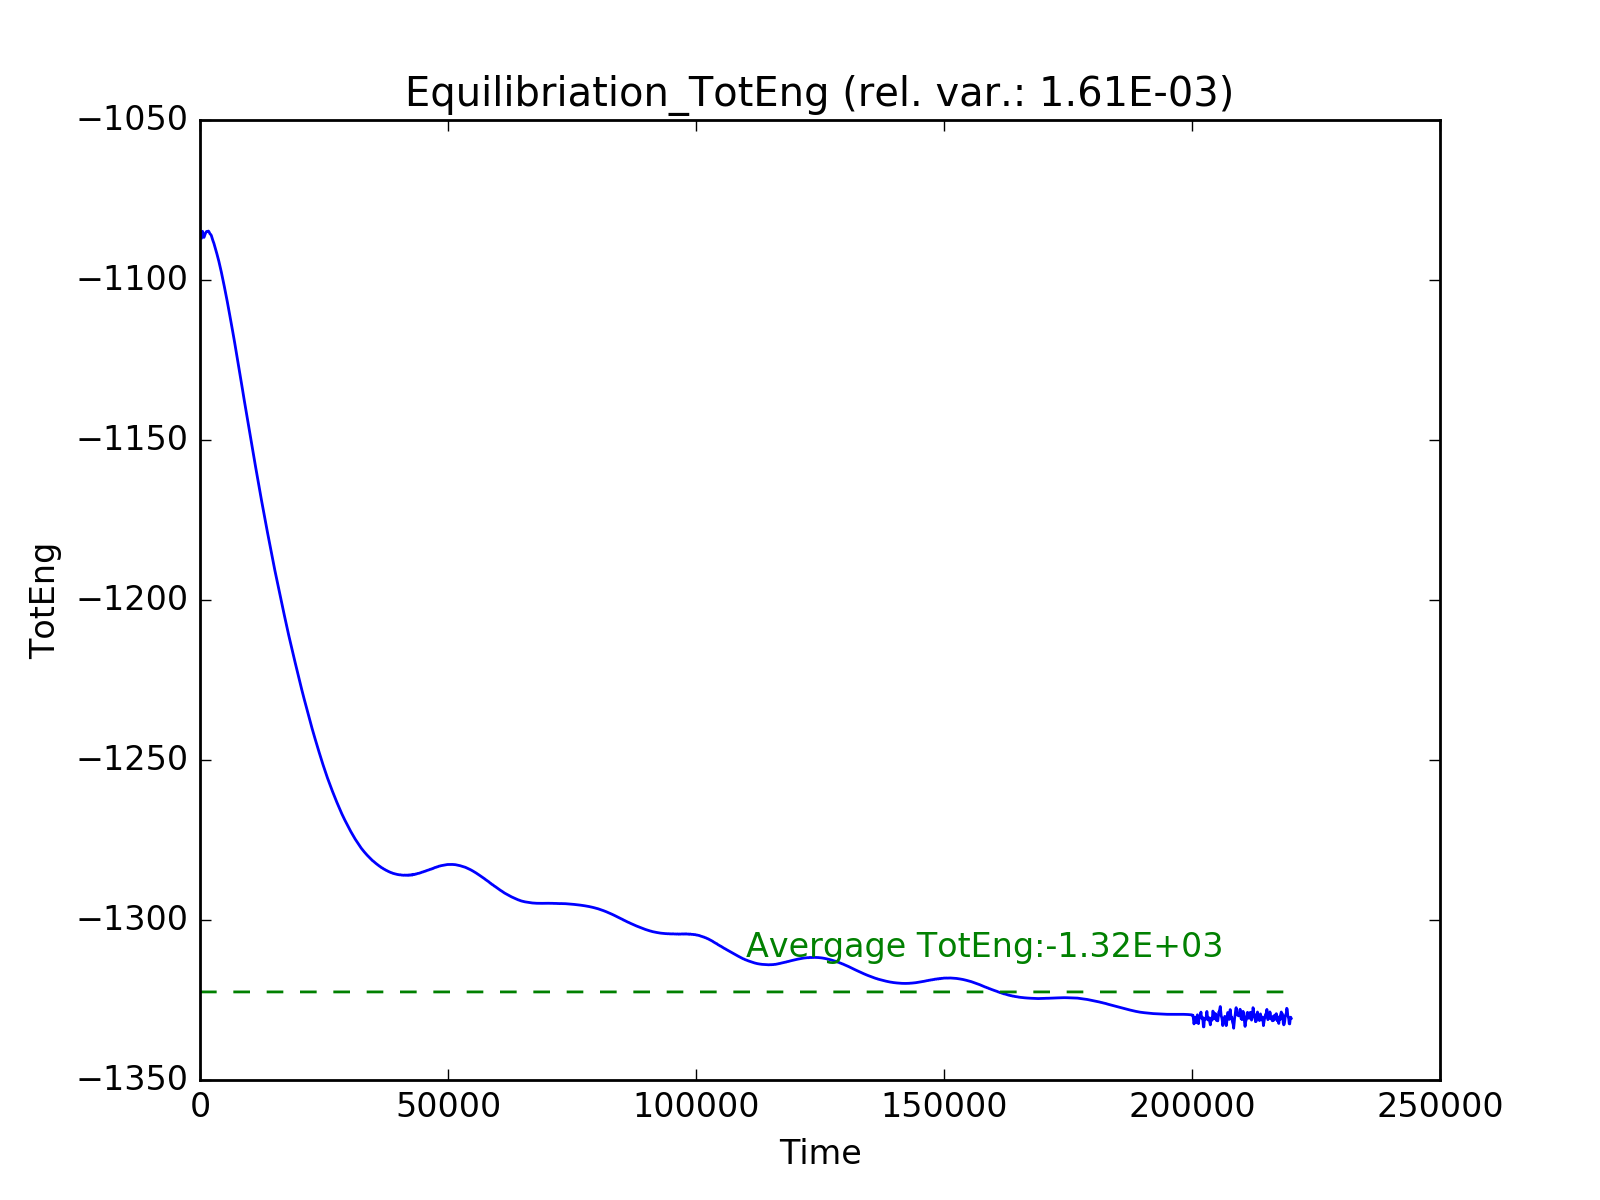
\includegraphics[width=0.5\textwidth]{\fullpathpartone/plots/CV/equi_TotEng.png}~
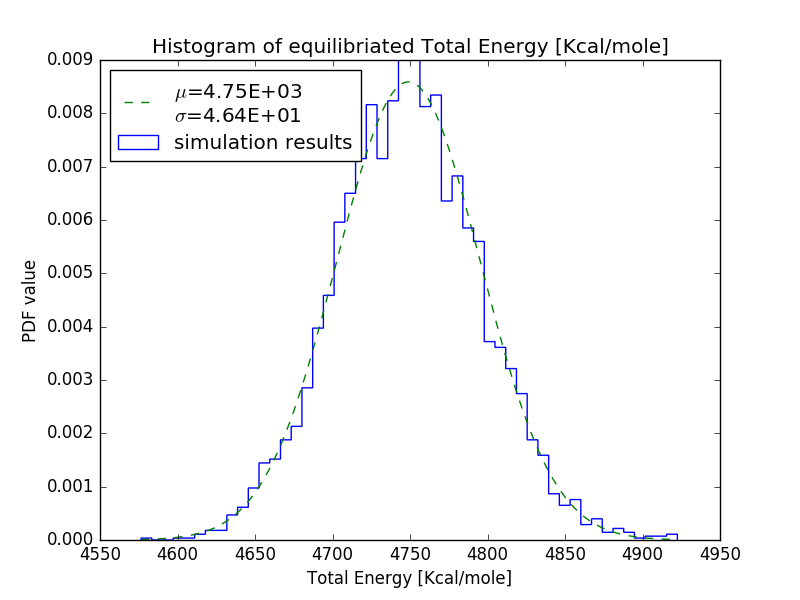
\includegraphics[width=0.5\textwidth]{\fullpathpartone/plots/CV/hist_equi_TotEng.png}
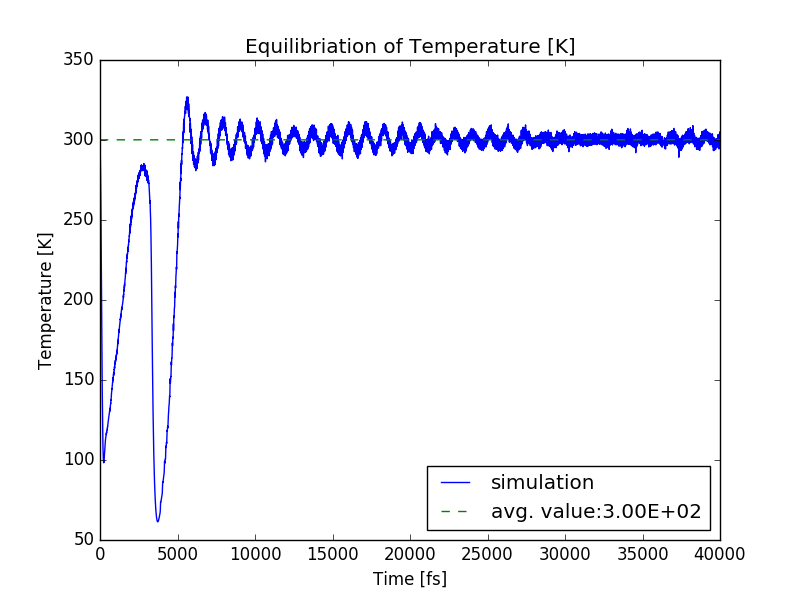
\includegraphics[width=0.5\textwidth]{\fullpathpartone/plots/CV/equi_Temp.png}~
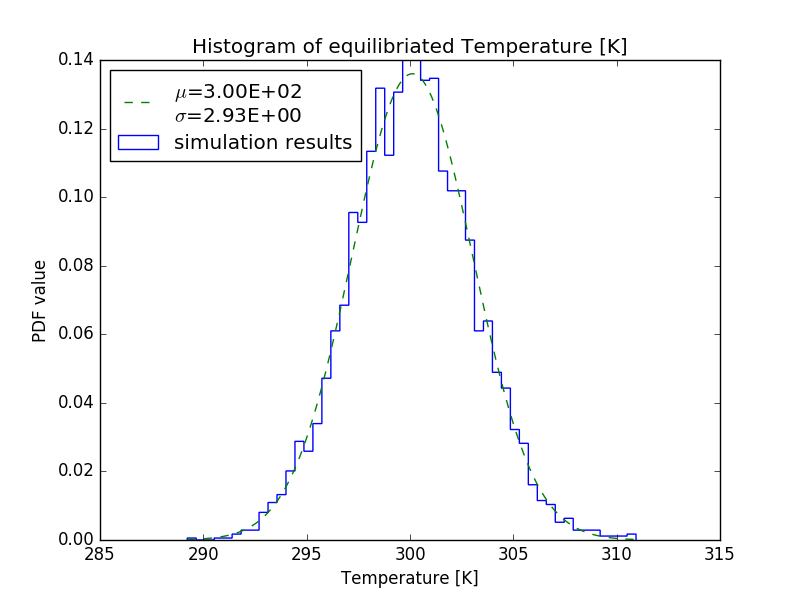
\includegraphics[width=0.5\textwidth]{\fullpathpartone/plots/CV/hist_equi_Temp.png}
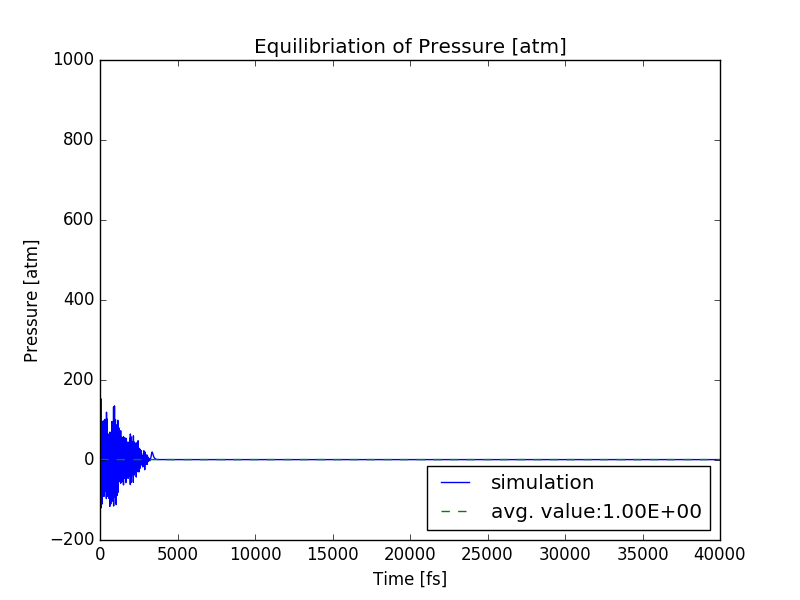
\includegraphics[width=0.5\textwidth]{\fullpathpartone/plots/CV/equi_Press.png}~
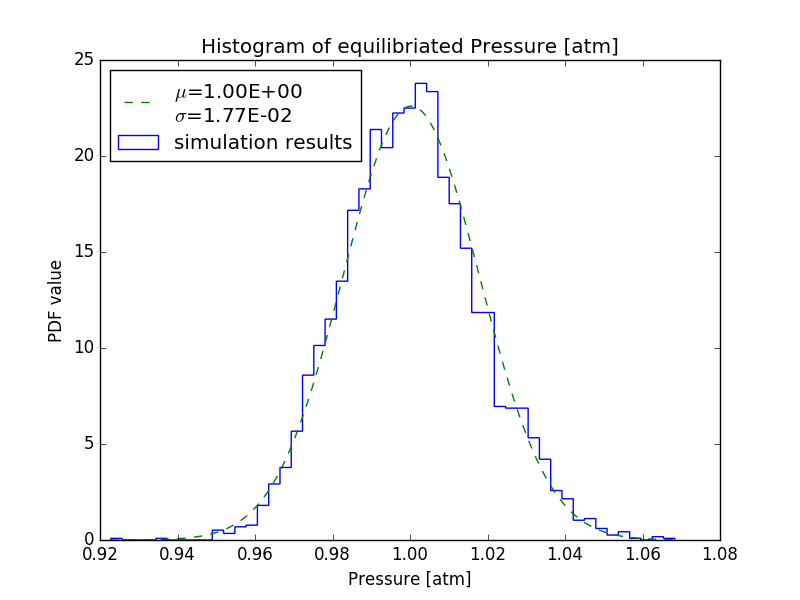
\includegraphics[width=0.5\textwidth]{\fullpathpartone/plots/CV/hist_equi_Press.png}
\caption[aaa]{Equilibriation of the system under NPT-Ensemble. The left part shows the development of thermodynamic quantities over time, the right figures show the distribution of those quantities after equilibration has been reached. Both the target Temperature and target Pressure have been reached with an acceptable standard deviation.}
\label{fig:p1_CV_equi_NPT}
\end{figure}
\end{center}

\begin{center}
\begin{figure}[h]
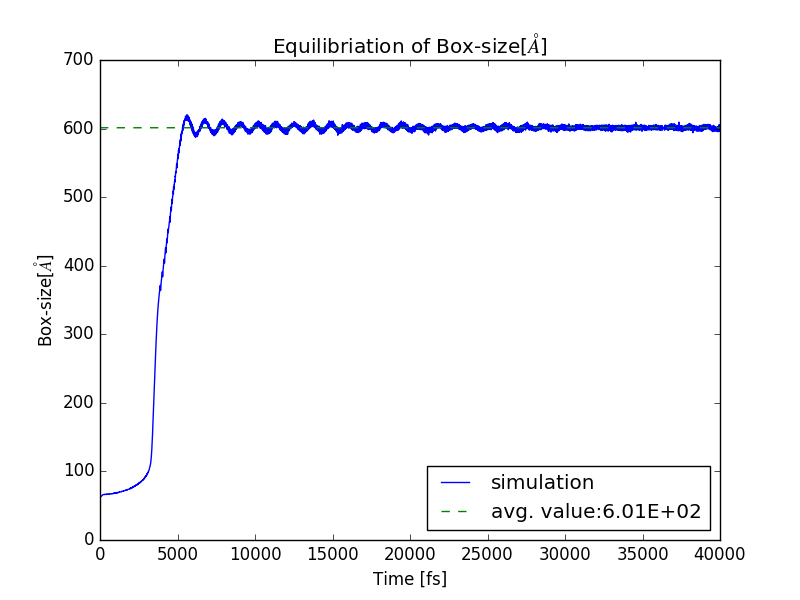
\includegraphics[width=0.5\textwidth]{\fullpathpartone/plots/CV/equi_Lx.png}~
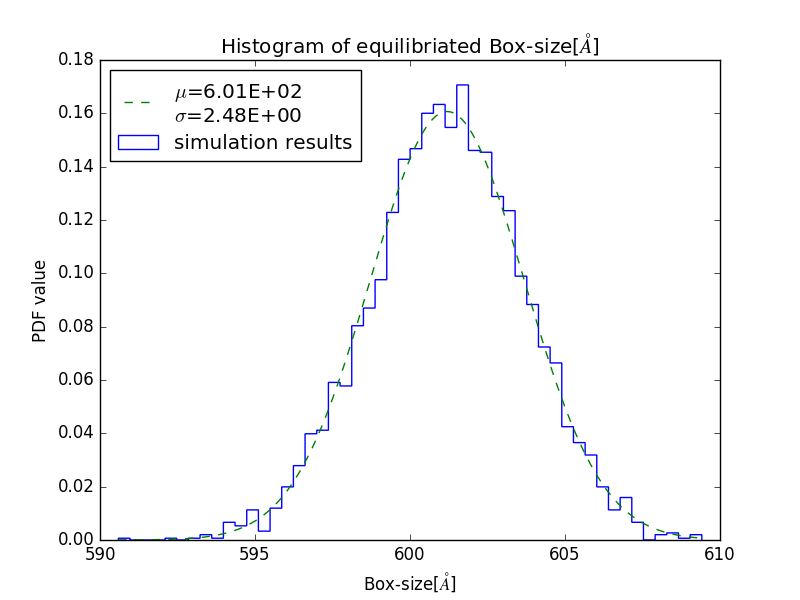
\includegraphics[width=0.5\textwidth]{\fullpathpartone/plots/CV/hist_equi_Lx.png}
\caption[aaa]{Estimation of the equilibrium Box length under the NPT ensemble. An equilibrated  value of $601~\AA$ is obtained with a standard deviation of $2.48 \AA$.}
\label{fig:p1_CV_equi_NPT_lx}
\end{figure}
\end{center}


\subsubsection{Estimation of specific heat capacity}
The specific heat capacity $C_v=\left(\frac{\partial E}{\partial T}\right)_{V,N}$ can, according to the instruction be written as a function of the total energy variance: $C_v=\frac{<E^2>-<E>^2}{k_B*T^2}$. I, however had problems with this formula. Even a short dimension analysis doesn't fit: $\frac{ {(kJ)}^2     }{ (\frac{kJ}{K}) {(K)}^2 } \neq \frac{kJ}{kg K}$.
However, one can also get a good approximation of $C_V$ by using a finite difference approach.
I did a central difference around $300.15~K$ with a stencil width of $1~K$ and obtained a value of $0.1516~\frac{kJ}{kg K}$, which coincides perfectly with the literature.
The input-files for this task were \href{\pathpartone/in.CV_NVT_plus}{in.CV\_NVT\_plus}, post-processing was done via \href{\pathpartone/postprocess_NVT.sh}{postprocess\_NVT.sh} and the finite difference approximation was carried out via \href{\pathpartone/calc_CV.py}{calc\_CV.py}.









\section{Phase transition of Krypton}


For the phase transition analysis, simulations between $25~K$ and $230~K$ have been carried out with a temperature-step of $1~K$. Each time the final configuration is written to a file and read by the subsequent simulation as a initial configuration.\\
The input-files are \href{\pathpartone/in.phasetrans}{in.phasetrans} for the first simulation and \href{\pathpartone/in.phasetrans_template}{in.phasetrans\_template} for all following.\\
The results are post-processed via \href{\pathpartone/postprocess_phasetrans.py}{postprocess\_phasetrans.py} and plotted via \href{\pathpartone/plot_phasetrans.py}{plot\_phasetrans.py}.\\
For the non-dimensionalization, the equilibrium box length is read from the logfile for each temperature.\\
Figure~\ref{fig:p1_phasetransition_dens} show the equilibrated density as a function of the equilibrated temperature. Two phase transitions at $\sim130~K$ and $\sim177~K$. 



\begin{center}
\begin{figure}[h]
\includegraphics[width=0.5\textwidth]{\fullpathpartone/plots/phasetrans/Density.png}~
%\includegraphics[width=0.5\textwidth]{\fullpathpartone/plots/phasetrans/red_Density.png}
\includegraphics[width=0.5\textwidth]{\fullpathpartone/plots/phasetrans/detail1/Density.png}~
%\includegraphics[width=0.5\textwidth]{\fullpathpartone/plots/phasetrans/detail1/red_Density.png}
\includegraphics[width=0.5\textwidth]{\fullpathpartone/plots/phasetrans/detail2/Density.png}~
%\includegraphics[width=0.5\textwidth]{\fullpathpartone/plots/phasetrans/detail2/red_Density.png}
\caption[aaa]{Phase transition analysis of Krypton in NPT ensemble. Simulations have been carried out every $1~K$. As the first graph shows, we get 2 distinct phase transitions. The two graphs below show the transitions in greater detail. One can conclude, that the melting occurs at $\sim130~K$, and Boiling at $\sim177~K$.}
\label{fig:p1_phasetransition_dens}
\end{figure}
\end{center}








\FloatBarrier
\pagebreak
\chapter{Two-dimensional atomistic tensile test}
All files for this task are located in \href{\pathparttwo}{2\_Two-dimensional\_atomic\_tensile\_test}\\
First, a system of $30\times30\times1$ cells has been set up and equilibriated under Nose-barostat. Several different compitantions of $T_{damp}$ and $p_{damp}$ have been used to determine the influence of both. The input file was \href{\pathparttwo\in.equi_template}{in.equi\_template}.
The influence of the damping parameters on the equilibriation of the Potential Energy is visualized in Figure~\ref{fig:p2_dampstudy_PotEng}.
First of all, if the damping parameter, particularly the pressure damping parameter, is chosen too low, the simulation becomes unstable and crashes. This was e.g. the case for $p_{damp}=10~fs$.\\
What is more, the graph shows, that the choice of $T_{damp}$ effects the convergence properties. The value should not be chosen too small. The choice of $p_{damp}$ on the other hand, seems not to influecne the convergence of the potential energy greatly, as long as it is choses such that the simulation is stable.\\
Additionally, the convergence of the system Temperature w.r.t the damping parameters is provided in Figure~\ref{fig:p2_dampstudy_PotEng}.\\
One can observe, that a too big choice of $T_{damp}$ leads to spurious osciallations at the beginning of the simuklations and periodic oscilattions even in the equilibriates regime.\\

Based on Figures~\ref{fig:p2_dampstudy_PotEng} and \ref{fig:p2_dampstudy_Temp} the following choice is made: $T_{damp}=100~fs$, $p_{damp}=100~fs$.
The equilibrium configuration is plottedin Figure~\ref{fig:p2_equi_ovito}.

\begin{center}
\begin{figure}[h]
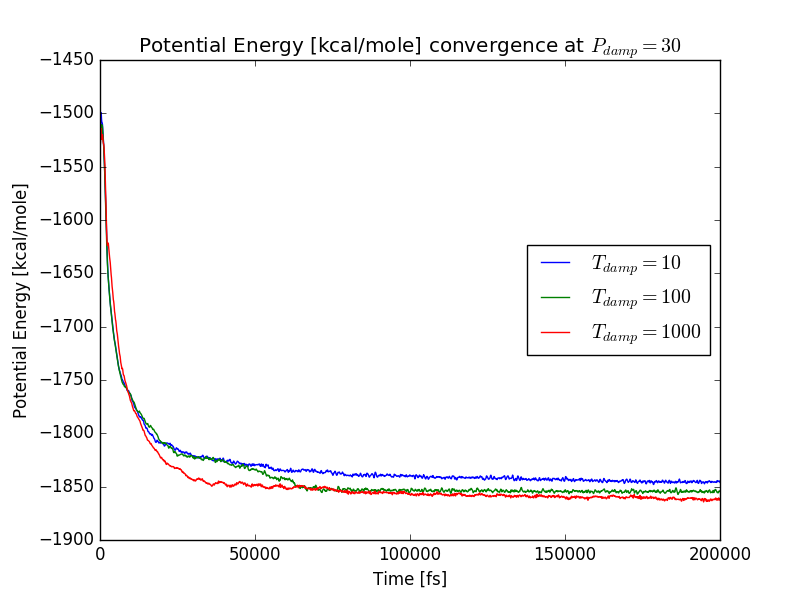
\includegraphics[width=0.5\textwidth]{\fullpathparttwo/plots/equi/dampstudy/NVT_PotEng_pdamp30.png}~
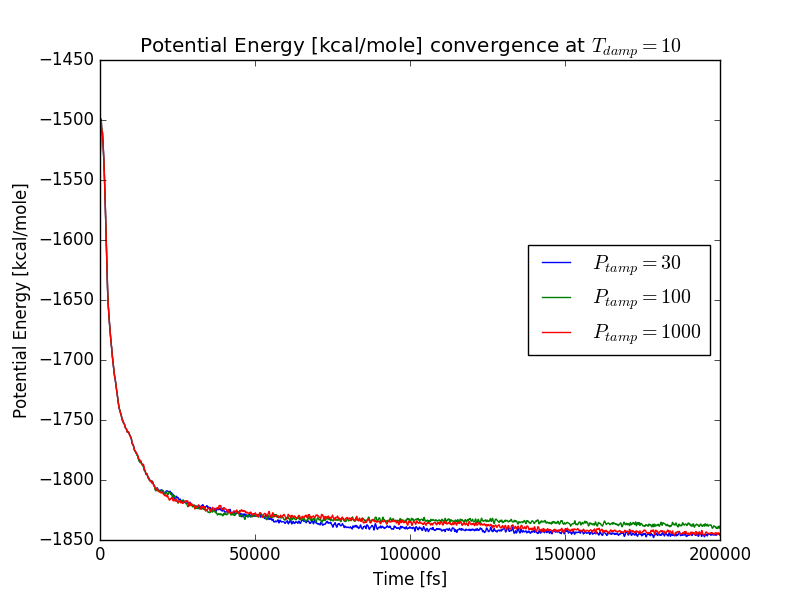
\includegraphics[width=0.5\textwidth]{\fullpathparttwo/plots/equi/dampstudy/NVT_PotEng_tdamp10.png}
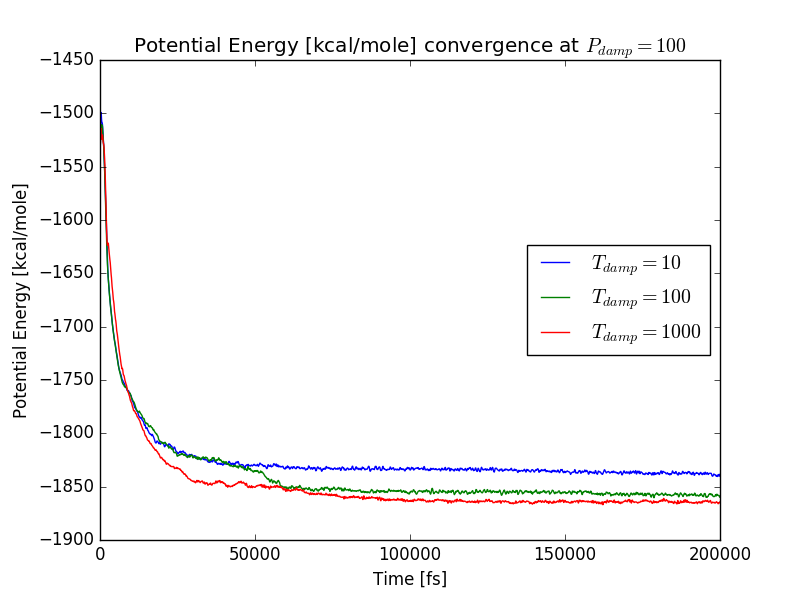
\includegraphics[width=0.5\textwidth]{\fullpathparttwo/plots/equi/dampstudy/NVT_PotEng_pdamp100.png}~
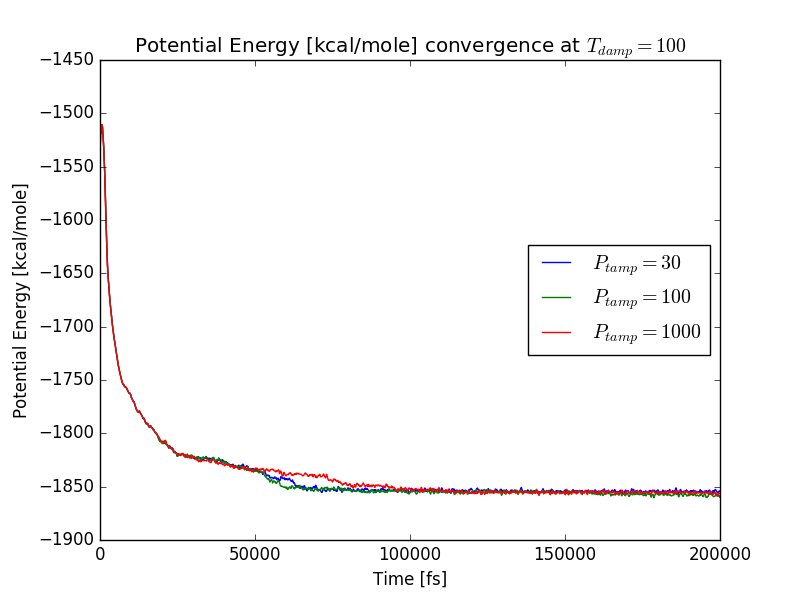
\includegraphics[width=0.5\textwidth]{\fullpathparttwo/plots/equi/dampstudy/NVT_PotEng_tdamp100.png}
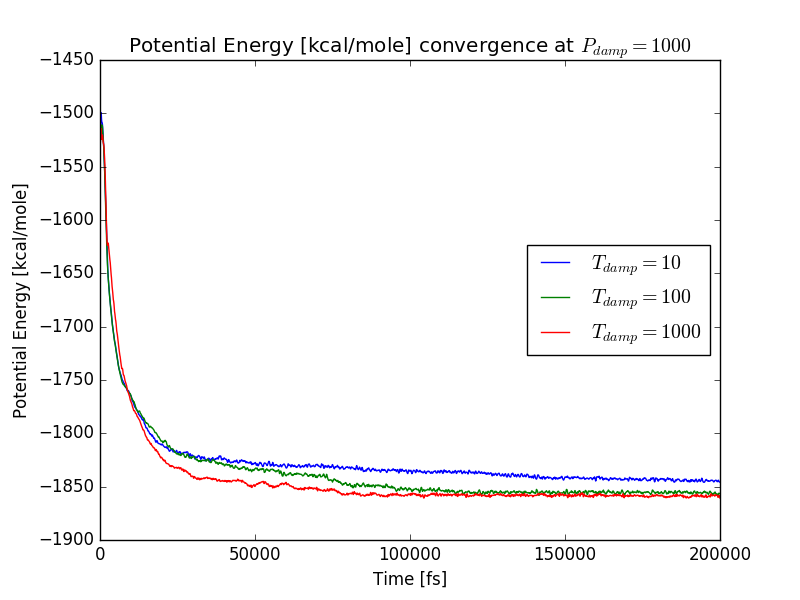
\includegraphics[width=0.5\textwidth]{\fullpathparttwo/plots/equi/dampstudy/NVT_PotEng_pdamp1000.png}~
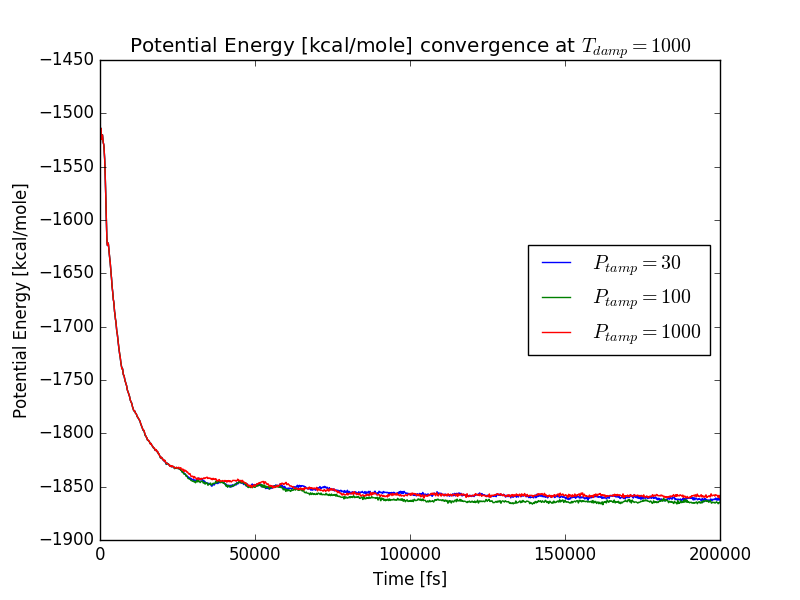
\includegraphics[width=0.5\textwidth]{\fullpathparttwo/plots/equi/dampstudy/NVT_PotEng_tdamp1000.png}~
\caption[aaa]{Influence of the damping parameters on the convergence of the potential energy. The plots on the left show a variation of $T_{damp}$ under constant values of $p_{damp}$, the plots on the left show a variation of $p_{damp}$ under constant values of $T_{damp}$.}
\label{fig:p2_dampstudy_PotEng}
\end{figure}
\end{center}

\begin{center}
\begin{figure}[h]
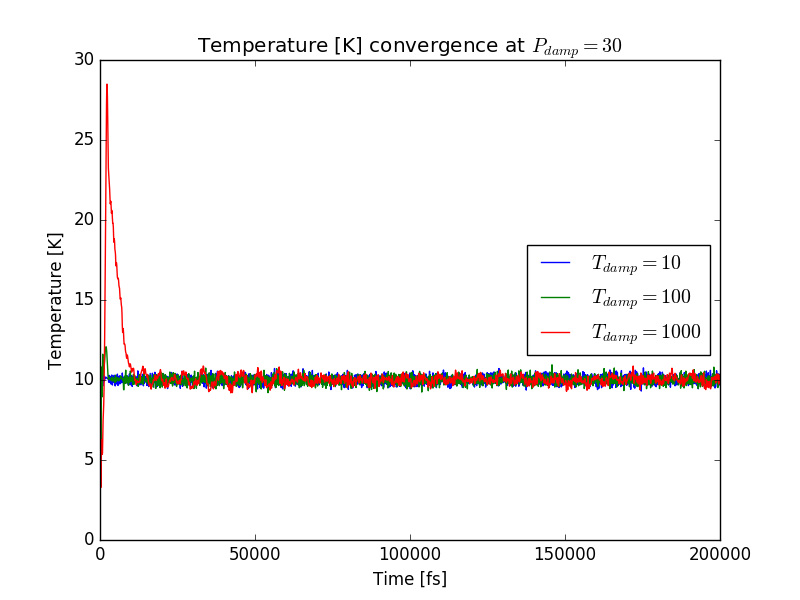
\includegraphics[width=0.5\textwidth]{\fullpathparttwo/plots/equi/dampstudy/NVT_Temp_pdamp30.png}~
\includegraphics[width=0.5\textwidth]{\fullpathparttwo/plots/equi/dampstudy/NVT_Temp_tdamp10.png}
\includegraphics[width=0.5\textwidth]{\fullpathparttwo/plots/equi/dampstudy/NVT_Temp_pdamp100.png}~
\includegraphics[width=0.5\textwidth]{\fullpathparttwo/plots/equi/dampstudy/NVT_Temp_tdamp100.png}
\includegraphics[width=0.5\textwidth]{\fullpathparttwo/plots/equi/dampstudy/NVT_Temp_pdamp1000.png}~
\includegraphics[width=0.5\textwidth]{\fullpathparttwo/plots/equi/dampstudy/NVT_Temp_tdamp1000.png}~
\caption[aaa]{Influence of the damping parameters on the convergence of the system temperature. The plots on the left show a variation of $T_{damp}$ under constant values of $p_{damp}$, the plots on the left show a variation of $p_{damp}$ under constant values of $T_{damp}$.}
\label{fig:p2_dampstudy_PotEng}
\end{figure}
\end{center}


\begin{center}
\begin{figure}[h]
\includegraphics[width=0.5\textwidth]{\fullpathparttwo/dump/equi/initial.png}~
\includegraphics[width=0.5\textwidth]{\fullpathparttwo/dump/equi/equilibrium.png}
\caption[aaa]{Initial(left) and equilibriated configuration(right) of the 2D-Krypton system. Thej atom radius is up to scale.}
\label{fig:p2_equi_ovito}
\end{figure}
\end{center}


\begin{center}
\begin{figure}[h]
\includegraphics[width=0.5\textwidth]{\fullpathparttwo/plots/stressx_strain.png}~
\includegraphics[width=0.5\textwidth]{\fullpathparttwo/plots/stressy_strain.png}
\caption[aaa]{Stress in x direction(left) and y-direction(right) as a function of the strain in x-direction. Clearly, the material begins to fail at a strain of approximately $0.2$. }
\label{fig:p2_stress_strain_relation}
\end{figure}
\end{center}



\end{document}